% BESCHREIBUNG DER DOCUMENTCLASS
% a4paper 	-	weil wir ein Din-A4-Dokument benutzen.
% 12pt		-	Schriftgröße von 12 Punkt.
% listof=totoc 	-	heisst, dass das Tabellenverzeichnis (\listoftables) & das Abbildungsverzeichnis (\listoffigures) im Inhaltsverzeichnis aufgenommen werden.
% bibtotoc		-	Das Literaturverzeichnis wird ins Inhaltsverzeichnis aufgenommen.
% scrreprt		-	Das Template für diese Dokument ist ein KOMA-Script Report

\documentclass[a4paper, 12pt, hidelinks, listof=totoc, listoftables=totoc, bibliography=totoc]{scrreprt}

\usepackage{lmodern}									% Modernes Lateinisches Schriftbild benutzen
\usepackage[T1]{fontenc}								% Schriftbild glätten
\usepackage[utf8]{inputenc}								% UTF-8 als input encoding nutzen
\usepackage[ngerman]{babel}								% Deutsche Silbentrennung
\usepackage[babel, german=quotes]{csquotes}
\usepackage{xcolor}										% Damit man Farben benutzen kann
\usepackage{setspace}									%
\usepackage[a4paper]{geometry}							%
\geometry{left=25mm, right=25mm, top=25mm, bottom=25mm}	% Seitenränder setzen
\usepackage{titlesec}									%
\usepackage{graphicx}									%
\usepackage{graphics}									%
\usepackage{listings}
\usepackage{alltt}
\usepackage{nameref}\lstset{
  literate={ö}{{\"o}}1
           {ä}{{\"a}}1
           {ü}{{\"u}}1
           {Ö}{{\"O}}1
           {Ä}{{\"A}}1
           {Ü}{{\"U}}1
           {ß}{{\ss}}1
}
\usepackage{hyperref}									% für Hyperlinks
\usepackage{url}										% um lange URLs darzustellen
%\usepackage{amsmath}									% für mathematische Formeln
%\usepackage{subfigure}									% eine Möglichkeit, um Bilder nebeneinander zu plazieren
%\usepackage{subcaption}
\usepackage{subfig}										% um Bilder nebeneinander zu plazieren
\usepackage[font=footnotesize]{caption}					% nötig, um die Font-Größe für Captions festzulegen


% Bibliographie mit biblatex/biber
\usepackage[backend=biber, style=alphabetic]{biblatex}
\addbibresource{biblio_scalajs.bib}


\graphicspath{{images/}}


%\definecolor{mid-red}{RGB}{224,0,0}
%\definecolor{mid-green}{RGB}{0,160,0}
%\definecolor{dark-blue}{RGB}{0,0,160}
\definecolor{mid-gray}{RGB}{127,127,127}
\definecolor{light-gray}{RGB}{244,244,244}
%\colorlet{keyword}{dark-blue}
%\colorlet{string}{mid-red}
%\colorlet{comment}{mid-green}
\colorlet{keyword}{black}
\colorlet{string}{black}
\colorlet{comment}{black}
\colorlet{linennumber}{mid-gray}
\colorlet{background}{light-gray}


% Sprachdefinitionen für Listings
\lstdefinelanguage{Scala}{
  morekeywords={
    abstract,case,catch,class,def,do,else,extends,false,final,finally,for,%
    forsome,if,implicit,import,lazy,match,mixin,new,null,object,override,%
    package,private,protected,requires,return,sealed,super,this,throw,trait,%
    true,try,type,val,var,while,with,yield%
  },
  otherkeywords={=>,<-,<\%,<:,>:,\#,@},
  sensitive=true,
  morecomment=[l]{//},
  morecomment=[s]{/*}{*/},
  morestring=[b]",
  morestring=[b]',
  morestring=[b]"""
}
\lstdefinelanguage{JavaScript}{
  morekeywords={
    break,case,class,catch,const,continue,debugger,default,delete,do,else,%
    export,extends,finally,for,function,if,import,in,instanceof,let,new,%
    return,super,switch,this,throw,try,typeof,var,void,while,with,yield%
    null,true,false,undefined,NaN%
  },
  sensitive=true,
  morecomment=[l]{//},
  morecomment=[s]{/*}{*/},
  morestring=[b]",
  morestring=[b]'
}
\lstdefinelanguage{HTML5}{
  language=html,
  tagstyle=\bfseries\color{keyword},
  morecomment=[s]{<!--}{-->},
  morestring=[b]",
  morestring=[b]'
}

% Styles für Listings
\lstdefinestyle{colored}{
  keywordstyle=\bfseries\color{keyword},
  commentstyle=\itshape\color{comment},
  stringstyle=\color{string}
}
\lstdefinestyle{uncolored}{
  keywordstyle=\bfseries,
  commentstyle=\itshape,
  stringstyle=\ttfamily
}
\lstdefinestyle{numbered}{
  numbers=left,
  numberstyle=\tiny\color{linennumber}
}
\lstdefinestyle{unnumbered}{
  numbers=none
}
\lstdefinestyle{framed}{
  backgroundcolor=\color{background}
}
\lstdefinestyle{unframed}{
  backgroundcolor=
}
\lstdefinestyle{basic}{
  basicstyle={\ttfamily\singlespacing\footnotesize}, 	% andere Font-Größen: \scriptsize \footnotesize \small
  showstringspaces=false,
  breaklines=true,
  breakatwhitespace=true,
  style=unnumbered,
  captionpos=b,
  %belowcaptionskip=4pt,
  literate={`}{{\`{}}}1			% for proper backticks
}
\lstdefinestyle{standard}{
  style=basic,
  style=colored,
  style=framed
}
\lstdefinestyle{standardnocol}{
  style=basic,
  style=uncolored,
  style=unframed
}
\lstdefinestyle{htmlnocol}{
  tagstyle=\bfseries
}
\lstdefinestyle{inline}{
  basicstyle={\ttfamily\small},
  breakatwhitespace=false
}
\lstdefinestyle{snippet}{
  aboveskip=-5pt,
  belowskip=0pt
}

% Default-Style für Listings. Kann überall im Text analog geändert werden.
\lstset{ style=standard }

% Kurzbefehle für Inline-Code.
\newcommand{\code}[1]{\lstinline[language=Scala, style=inline]|#1|}
\newcommand{\scala}[1]{\lstinline[language=Scala, style=inline]|#1|}
\newcommand{\js}[1]{\lstinline[language=JavaScript, style=inline]|#1|}
\newcommand{\html}[1]{\lstinline[language=HTML5, style=inline]|#1|}


%Arial nutzen wer will...
%\renewcommand{\rmdefault}{phv} % Arial
%\renewcommand{\sfdefault}{phv} % Arial

% FORMATIERUNG DER ÜBERSCHRIFTEN ANFANG
	% Überschriftenformatierung
	% Erklärung: \titleformat{Überschriftenklasse}[Absatzformatierung]{Textformatierung}{Numerierung}{Abstand zwischen Numerierung und Überschrift}{Code davor}[Code danach]
	% 1. Ebene chapter
	\titleformat{\chapter}[hang]{\Large\bfseries}{\thechapter\quad}{0pt}{}
	% 2. Ebene -- section
	\titleformat{\section}[hang]{\large\bfseries}{\thesection\quad}{0pt}{}
	% 3. Ebene -- subsection
	\titleformat{\subsection}[hang]{\bfseries}{\thesubsection\quad}{0pt}{}
	% 4. Ebene -- subsubsection
	\titleformat{\subsubsection}[hang]{\bfseries}{\thesubsubsection\quad}{0pt}{}

	% Platz um die Überschriften
	% Erklärung: \titlespacing{Überschriftenklasse}{Linker Einzug}{Platz oberhalb}{Platz unterhalb}[rechter Einzug]
	\titlespacing{\chapter}{0pt}{0pt}{10pt}
	\titlespacing{\section}{0pt}{20pt}{10pt}
	\titlespacing{\subsection}{0pt}{20pt}{10pt}
% FORMATIERUNG DER ÜBERSCHRIFTEN ENDE

% FORMATIERUNG FLIESSTEXT ANFANG
	% Absatzeinrueckung unterdruecken
	\setlength{\parindent}{0pt}
	% Abstand zwischen zwei Absaetzen setzen
	\setlength{\parskip}{6pt}
	% Zeilenabstand
	% Optionen: \singlespacing , \onehalfspacing , \doublespacing
	\onehalfspacing
% FORMATIERUNG FLIESSTEXT ENDE

% EIGENE KOPFZEILE ANFANG
	\usepackage{scrpage2}
	\clearscrheadfoot
	\ihead[\footnotesize{\textnormal{\headmark}}]{\footnotesize{\textnormal{\headmark}}}
	\ohead[\footnotesize{\pagemark}]{\footnotesize{\pagemark}}
	\automark{chapter}
	% Numerierung nur bis subsection
	\setcounter{secnumdepth}{2}
% EIGENE KOPFZEILE ENDE


% Wird gebraucht für die Titelseite...
\newcommand{\RM}[1]{\MakeUppercase{\romannumeral #1{}}}

% Erstellung eines Index
\makeindex

%%%%%%%%%%%%%%%%%%%%%%%%%%%%%%%%%%%%%%%%%%%%%%%%%%%%%%%%
% BEGIN DOCUMENT // HIER FÄNGT DER INHALT AN
%%%%%%%%%%%%%%%%%%%%%%%%%%%%%%%%%%%%%%%%%%%%%%%%%%%%%%%%
\begin{document}

% Import der Titelseite aus dem Ordner "title".
\begin{titlepage}
\begin{center}
	\begin{figure}[!h]
		
\includegraphics[scale=1]{./title/Beuth_Logo_horizontal.jpg}
	\end{figure}

	% vertikaler Zwischenraum
	\vspace{15mm}

	\large
		\textbf{Fachbereich \RM{6} $\cdot$ Informatik und Medien\\[3mm]
		Studiengang Medieninformatik}\\

	\vspace{15mm}

	\Large
		\textbf{Bachelorarbeit}\\[5mm]
	\normalsize
		zur Erlangung des akademischen Grades\\
		Bachelor of Science (B.Sc.)\\

	\vspace{15mm}

	\huge
		\textbf{Evaluierung von Scala.js \\
		für interaktive Weboberflächen }\\ [0,5cm]
	
	\Large
		\textbf{Untertitel ... TODO}\\[2cm]

	\normalsize
	\begin{tabular}{rl}
		vorgelegt von: & Sebastian Dassé \\
		Matrikelnummer: & 791537 \\
		am: & \today \\
		& \\
		Betreuer: & Prof. Christoph Knabe\\
		Gutacher: & Prof. Dr. Elmar Böhler\\
	\end{tabular}\\
\end{center}
\end{titlepage}

% Keine Kopfzeile im Inhaltsverzeichnis
\pagenumbering{gobble}

% Inhaltsverzeichnis erstellen
\tableofcontents

% Neue Seite.
\newpage

% Kopfzeile an
\pagestyle{scrheadings}

%Seitennummern anfangen
\pagenumbering{arabic}



% % % % % % % % % % % % % % % % % % % % % % % % % % % % % % % %
\chapter{Einleitung}

%TODO Zitate checken, ggf. ergänzen um "`vgl."'

% evtl. hilfreich:  D:\UNI\2014-SoSe\GWAGWA_Themenfindung_Gliederung_Schreibstil.pdf

\section{Motivation}

% siehe jeweils Einleitung von Doeraene 2013 und Haoyi 2015

(- Weboberflächen basieren auf HTML und CSS)
- von modernen Webseiten wird in zunehmendem Maße viel Interaktionsmöglichkeiten/Interaktivität erwartet, im Vergleich zu älteren/klassischen statischen Webseiten eher Desktopanwendungen ähnlich ... (man spricht deshalb auch von Rich Internet Applications) (also: für Interaktivität auf Clientseite) existiert als De-facto-Standard JavaScript (von allen Browsern ohne Plugins unterstützt (alle Browser haben einen JavaScript-Interpreter)
-->  \url{http://w3techs.com/technologies/overview/client_side_language/all}
; mögliche Alternativen mit Plugins: Flash, Java Applets, MS Silverlight; aber beide Techniken immer weniger gebräuchlich, weil: Flash Video-Player seit HTML5 video Bedeutungsverlust, Flash-Format für animierte Inhalte ersetzt durch JS-Bibliotheken wie etwa jQuery und HTML5-Techniken wie <canvas>, SVG und WebGL, Silverlight deprecated, Applets lange Ladezeiten), verlieren aber zunehmend an Bedeutung  -->  Diagramm:   \url{https://www.google.com/trends/explore#q=adobe+flex,microsoft+silverlight,java+applet,HTML5,gwt}
- JavaScript aus verschiedenen Gründen problematisch
  - nicht typsicher (-> Fehler zur Laufzeit)
  - viele kontraintuitive Besonderheiten der Sprache auf die zu achten ist -> sind zwar dokumentiert, aber erschweren das Programmieren und führen zu schwer zu findenden Fehler (wie dem notorischen Fehlertext in der Browserkonsole: \js{undefined is not a function})
  - relativ "`verbose"'/geschwätzig
  - schlechte Wartbarkeit
  - aufwendiges Refactoring

JavaScript wurde 1995 von Brendan Eich für Netscape innerhalb von zehn Tagen entwickelt\cite{wikipedia.JS}. 
War der Einsatzzweck der Sprache zu dieser Zeit in erster Linie der, statische Webseiten durch interaktive Elemente attraktiver zu machen, so werden heute komplexe Webanwendungen in JavaScript geschrieben. Hierfür kommt häufig eine immer breiter werdende Palette an JavaScript-Frameworks zum Einsatz, durch die auf strukturierende Hilfsmittel sowie auf eine erweiterte Standardfunktionalität zurückgegriffen werden kann. Das führt wiederum zu mehr Lernaufwand bei der Einarbeitung in diese Frameworks.

-->  \url{https://en.wikipedia.org/wiki/Comparison_of_JavaScript_frameworks}


Liy Haoyi, Mitarbeiter beim Scala.js-Projekt und Autor des E-Books "`Hands-on Scala.js"' bringt die Motivation, für Scala.js auf den Punkt: "`At this point, all of Google, Facebook, and Microsoft have all announced work on a typed variant of Javascript. These are not academic exercises: Dart/AtScript/Flow/Typescript are all problems that solve a real need, that these large companies have all faced once they've grown beyond a certain size. Clearly, Javascript isn't cutting it anymore, and the convenience and "`native-ness"' of the language is more than made up for in the constant barrage of self-inflicted problems. Scala.js takes this idea and runs with it!"'\cite[\#TheLanguage]{haoyi.HOS}




>> andere Sprachen die nach JavaScript kompilieren

JavaScript wird schon bezeichnet als Assembler für das Internet ("`assembly language for the web"') bzw. Virtual Machine des Internets ("`VM of the web"', Douglas Crockford)
  -->  \url{http://www.hanselman.com/blog/JavaScriptIsAssemblyLanguageForTheWebSematicMarkupIsDeadCleanVsMachinecodedHTML.aspx}
  --> \url{http://www.hanselman.com/blog/JavaScriptIsAssemblyLanguageForTheWebPart2MadnessOrJustInsanity.aspx}
  - JavaScript ist eine Plattform\cite{doeraene2015.SSP}

zwei Kategorien
1. ausgehend von JavaScript Verbesserung der Sprache durch angenehmere Syntax oder statische Typisierung
	- CoffeeScript (nicht getypt)
	- TypeScript (getypt, Obermenge von JavaScript, d.h. JS ist immer auch TS)
	Kritik von Doeraene: -> wenig Gewinn an Expressivität
2. andere statisch getypte Sprachen (extra neu entwickelte oder existierende), die nach JS kompilieren
	Dart, GWT (Java -> JS)
	Kritik von Doeraene: -> schlechte Interop mit JavaScript-libs, weil JS values nicht als first-class objs der host lang
\cite[S. 1]{doeraene2013.TDI}

Interop mit JavaScript-libs wichtig: DOM, andere Libs
\cite[S. 1]{doeraene2013.TDI}





Code-Wiederverwendung
- traditionell verschiedene Sprachen für Client und Server
	- Client bei weitem dominiert von JavaScript (90 \% \cite{w3techs.CLI})
	- Server (PHP, Java u.a. \cite{w3techs.SRV})
- in dem Fall:
	- Mehrfachimplementierung von Algorithmen
	- Ajax-Aufrufe um Logik an einem Ort zu halten
- eine Sprache auf Client und Server: mit Node.js JavaScript, aber mit allen beschriebenen Problemen von JS








- nicht JavaScript verwenden -> man ist alle Probleme des Programmierens in JS los
- eine Sprache für beide Seiten, Client und Server, wünschenswert
  - auf Serverseite in der Regel andere Sprache wie Java, PHP, ... ???
  - Vorteile wären: Wiederverwendbarkeit von Code, Definition gemeinsamer Schnittstellen (in der Form bisher nicht möglich)

- Scala.js bringt Scala (bisher auf Basis der JVM) auf die Client-Seite:
  - es kann in Scala entwickelt werden
  - Scala-Code wird nach JavaScript als Zielsprache übersetzt
  - Compiler, Ökosystem aus Bibliotheken und Tools/Entwicklungswerkzeugen



\section{Zielstellung / Aufgabenstellung}

Ziel: untersuchen, wie gut Scala.js zur Entwicklung von Weboberflächen geeignet ist
Fragen:
  - entwickelt man robuster?
  - steigert es die Code-Qualität?
  - entwickelt man schneller?
  - ist es angenehm, mit Scala.js zu entwickeln?
  - kann das Resultat mit herkömmliche Weise mit JavaScript entwickelten Anwendungen mithalten oder übertrifft es sie sogar?
  - entsprechend: ist das Ergebnis performant genug?
  - aus Benutzersicht: wie schnell lädt die Seite?

Anhand verschiedener kleinerer Anwendungen / anhand der Anwendung ... soll untersucht werden, wie gut Scala.js den heutigen Anforderungen an die Frontend-Entwicklung gerecht wird.


Abgrenzung:

	NICHT IM FOKUS: Browser-Kompatibilität
	NICHT IM FOKUS: Server mit Datenbank
	NICHT IM FOKUS:  ist es gut/schlecht viel clientseitigen JS-Code zu haben - möglicherweise besser, mehr statisches HTML zu serven, und nur Teile dynamisch durch JS erzeugen zu lassen?


\section{Aufbau der Arbeit}

TODO






















% % % % % % % % % % % % % % % % % % % % % % % % % % % % % % % %
\chapter{Technikvorstellung/fachliches Umfeld/Grundbegriffe (3)}

\section{Scala (1.5)}

%-->  \cite{fiedler2011.ELS} S. 5-8

%TODO kürzen!

Scala ist eine moderne Multiparadigmen-Programmiersprache, die objektorientierte und funktionalen Programmierkonzepte mit einer statischen Typisierung verbindet. Sie wird seit 2001 federführend von Martin Odersky an der École polytechnique fédérale de Lausanne (EPFL) entwickelt und wurde erstmals 2004 öffentlich vorgestellt.
%"`Scala smoothly integrates object-oriented and functional programming. It is designed to express common programming patterns in a concise, elegant, and type-safe way."'  --> \url{http://article.gmane.org/gmane.comp.lang.scala/17}
Seit der Gründung der Firma Typesafe 2011 durch Odersky und Jonas Bonér\footnote{Bonér ist der Autor von \textit{Akka}, einem Toolkit und einer Laufzeitumgebung zur Entwicklung fehlertoleranter nebenläufiger und verteilter Anwendungen. Es basiert auf einem Modell, bei dem \textit{Aktoren} genannte nebenläufige Einheiten durch Nachrichtenaustausch miteinander kommunizieren. Akka ist Teil der Typesafe-Plattform. \url{http://akka.io/}} erfährt die Entwicklung von Scala als Teil der \textit{Typesafe Reactive Platform} nun auch kommerzielle Unterstützung.
Hier wird unter anderem die IDE-Integration für Scala vorangetrieben und das Buildtool \textit{sbt} entwickelt.\cite{scala-lang2011.CSS} 

Scala verwendet eine prägnante, schlanke Syntax. So lässt sich etwa eine einfache Klasse als Einzeiler schreiben: \scala{class Foo(val bar: Int)}. Damit sind sowohl ein Konstruktor als auch die Instanzvariable (\scala{bar}) definiert. Dadurch sind Scala-Programme eher kurz. Ein Java-Programm lässt sich mit etwa der halben Anzahl an \textit{Lines of Code} in Scala formulieren. Das reduziert den Schreib- und Leseaufwand und die Gelegenheit Fehler zu machen.

Scala erlaubt es, auf einem relativ hohen Abstraktionslevel zu programmieren und macht es so erleichtert den Umgang mit komplexen Systemen.

Scala-Programme kompilieren zu Java-Bytecode und laufen auf der JVM\footnote{\textit{Java Virtual Machine}}. Ihre Performance ist mit der von Java-Programmen vergleichbar. Scala-Code kann Java-Code aufrufen. Dadurch hat der Scala-Programmierer\footnote{GENDERKLAUSEL: der Einfachheit halber wird im Text die männliche Form verwendet; natürlich ist auch die Programmiererin gemeint.} automatisch auch alle Libraries zur Verfügung. Scala-Code kann auch von Java-Code aufgerufen werden, aber hier sind manchmal einige Feinheiten zu beachten.\cite[S. 13 ff.]{odersky2008.PIS}

Der Einstieg in die Sprache Scala ist relativ einfach. Durch die Mächtigkeit der Sprachmittel und die Vielzahl der sich daraus ergebenden Möglichkeiten ist für eine tieferes Verständnis allerdings ein hoher Lernaufwand nötig.

%(>>Wurzeln: Syntax ähnlich Java, ML)


\subsection{Objektorientierung}

Scala ist eine rein objektorientierte Sprache: Jeder Wert ist ein Objekt. Das schließt auch numerische Werte und Funktionen ein, primitive Typen wie in Java existieren nicht. Doch die Objektorientierung geht sogar noch weiter: In Scala ist jede Operation ein Methodenaufruf. So ist \scala{1 + 2} der Aufruf der Methode \scala{+} an einer Instanz der Klasse \scala{Int} und könnte auch als \scala{1.+(2)} ausgedrückt werden. Konsequenterweise sind auch statische Methoden unbekannt. Stattdessen werden mit dem Schlüsselwort \scala{object} Singleton-Objekte definiert, die Methoden und Werte aufnehmen können, welche nicht Attribute der Instanz einer Klasse sind. Diese können entweder alleinstehend sein oder als sogenanntes Begleitobjekt (\textit{companion object}) einer gleichnamigen Klasse auftreten.

Benutzerdefinierte Typen lassen sich mithilfe von Klassen und \textit{Traits} definieren. Traits sind den Interfaces in Java ähnlich, sie können allerdings Implementierungen von Methoden und sogar Felder enthalten. Außerdem können Traits mehrfach beerbt werden (man spricht hierbei auch von \textit{mixin class composition}).

Die Modularisierung von Programmen funktioniert grundsätzlich ähnlich wie in Java, allerdings stellt Scala flexiblere und generischere Mittel zur Verfügung. Importe können grundstäzlich überall platziert werden. Dabei können neben Paketen und Paket-Membern auch Objekte importiert werden. Member können auch unter anderem Namen importiert werden, sei es um Namenskonflikte zu vermeiden oder um häufig verwendete Namen abzukürzen.
Pakete können, anders als in Java, beliebig verschachtelt werden. Die Zugriffsmodifizierer werden konsistenter und granularer als in Java gehandhabt. Beginnt etwa die Deklaration einer Methode mit \scala{private[this]}, so darf nur durch das Objekt selbst auf diese Methode zugegriffen werden.\cite[S. 9 f., S. 233 ff.]{odersky2008.PIS}\cite{scala-lang.ATS}

\subsection{Funktionale Programmierung}

%funktional (aber auch imperativ)

%Scala unterstützt funktionale Programmierung.
Scala ist eine vollständig funktionale Sprache.\footnote{Funktionale Programmierung basiert auf dem in den 1930er Jahren von Alonzo Church entwickelten Lambda-Kalkül. Dessen zentrale Idee besteht darin, dass Funktionen anonym definiert werden. Das Lambda-Kalkül ist Turing-vollständig, und somit gleich mächtig wie imperative Sprachen. Jedes imperative Programmierkonstrukt lässt sich demnach auch funktional ausdrücken.} Funktionen sind in Scala \textit{first-class values}, das heißt sie haben denselben Status wie alle anderen Daten. Sie können einer anderen Funktion als Parameter übergeben werden oder von einer anderen Funktion zurückgegeben werden. Diese "`andere"' Funktion bezeichnet man als Funktion höherer Ordnung. Funktionen können ineinander verschachtelt werden und anonym als \textit{Funktionsliterale} (oft auch Lambda-Funktionen genannt) verwendet werden.

Funktionen bilden Eingabewerte auf Ausgabewerte ab, ohne dabei den Zustand der Eingabewerte zu verändern. Man sagt: Sie sind frei von Nebenwirkungen (\textit{side effects}). Zusätzlich sind Funktionen referentiell transparent, das heißt sie liefern für gleiche Argumente immer das gleiche Ergebnis. Für jeden Eingabewert kann der Funktionsaufruf durch sein Resultat ersetzt werden, ohne dass sich dadurch die Semantik ändert. Durch diese Eigenschaften wird die funktionale Programmierung zunehmend attraktiv für den Einsatz in nebenläufigen Programmen. Einfach ausgedrückt: Werte die sich nie ändern müssen auch nicht synchronisiert werden.

Darüberhinaus kennt Scala \textit{Closures}, \textit{Currying} und \textit{List comprehensions}\footnote{in Scala: \textit{Sequence comprehensions}}.

Scala unterstützt zwar die nebenwirkungsfreie funktionale Programmierung mit unveränderlichen (\textit{immutable}) Daten, lässt einem aber die Wahl, gegebenenfalls im imperativen Stil zu programmieren.\cite[S. 6 ff.]{piepmeyer2010.GFP}\cite[S. 10 ff.]{odersky2008.PIS}

\subsection{Einheitliches statisches Typsystem}

Scala verfügt über ein ausdrucksstarkes einheitlich Typsystem mit einer gemeinsamen Superklasse \scala{Any} von der jede Klasse erbt. \scala{Any} hat exakt zwei direkte Subklassen: \scala{AnyVal} und \scala{AnyRef}. 

Von \scala{AnyVal} erben die neun Scala-eigene Werteklassen: \scala{Byte}, \scala{Short}, \scala{Char}, \scala{Int}, \scala{Long}, \scala{Float}, \scala{Double} und \scala{Boolean}, die den primitiven Typen in Java entsprechen\footnote{sie werden sogar zur Laufzeit durch primitive Java-Typen ersetzt} und \scala{Unit}, das etwa \scala{void} in Java entspricht. \scala{AnyRef}, die andere Subklasse von \scala{Any}, ist die Basisklasse für alle Referenzklassen. Auf der Java-Plattform ist \scala{AnyRef} nur ein Alias für die Klasse \scala{java.lang.Object}. 

Außerdem existieren noch zwei spezielle Klassen: \scala{Null} und \scala{Nothing}. \scala{Nothing} ist eine gemeinsame Subklasse jeder anderen Klasse. Dieser Typ kann keine Werte enthalten, wird aber benötigt um zum Beispiel den Typ der leeren Liste zu definieren: \scala{List[Nothing]}. Die Klasse \scala{Null} enthält \scala{null} als einzigen Wert und ist der Subtyp aller Rerenzklassen, also aller Klassen, die von \scala{AnyRef} erben.

Scala ist statisch typisiert, das bedeutet es findet eine Typprüfung zur Compile-Zeit statt. Daraus leiten sich sich verschiedene entscheidende vorteilhafte Eigenschaften ab. Ein Typ ist nichts anderes als die Festlegung des Wertebereichs und der möglichen Operationen für ein Objekt. Ist der Typ eines Objekts bekannt, so werden an ihm beispielsweise nie Methoden aufgerufen oder auf Attribute zugegriffen werden können, die er nicht besitzt. Solche Programmierfehler würde der Compiler melden und das Programm einfach nicht übersetzen. Mit der statischen Typprüfung sind demnach echte Garantien verbunden, die bestimmte Laufzeitfehler sicher ausschliessen, und zwar sicherer als jeder Unit-Test.

Diese Typsicherheit bedeutet auch eine größere Sicherheit beim Refactoring und eine deutlich stärkere Unterstützung durch IDEs: beim Refactoring, bei der komfortablen Quellcodenavigation (wie etwa das Springen zur Definition eines Werts) und durch typbasierte automatische Code-Vervollständigung. Nicht zuletzt ist Code automatisch besser dokumentiert, wenn die Typen der Attribute, Parameter und Funktionsrückgabewerte bekannt sind.

Trotz strenger Typisierung erlaubt Scala einen flexiblen Umgang mit seinen Typen. Durch ein System der automatischen Typableitung (\textit{Typinferenz}) werden redundante Typangaben vermieden und häufig kommen Deklarationen sogar ganz ohne explizite Typangaben aus. Der eingebaute Mechanismus des \textit{Pattern Matching}\footnote{raffinierte Form einer switch-Anweisung anhand der Struktur oder dem Typ eines Objekts} erlaubt einen sehr flexiblen Umgang mit streng getypten Werten.

Außerdem erlaubt Scala generische Klassen, innere Klassen, abstrakte Typen als Member, zusammengesetzte Typen (\textit{compound types}) und implizite Parameter.\cite[S. 16 ff., S. 205 ff.]{odersky2008.PIS}\cite[S. 113 ff.]{piepmeyer2010.GFP}\cite{scala-lang2011.CSS}

\subsection{Erweiterbarkeit}

Scala trägt die Erweiterbarkeit im Namen ("`scalable language"').
%"eine Sprache die mitwächst" ("a language that grows on you")
Die Sprache hat einen relativ kompakten Kern und liefert einen großen Umfang an Funktionalität in Form einer Standardbibliothek. Diese enthält unter anderem ein äußerst unfangreiches Collections-Framework, eine Mathematik-Bibliothek, Bibliotheken für reguläre Ausdrücke, zur XML-Manipulation, zur nebenläufigen Programmierung mit Futures und Promises und eine Aktoren-Bibliothek, welche Nebenläufigkeit durch Nachrichtenaustausch realisiert.\footnote{Einen guten Überblick über die Standardbibliothek bietet die API-Dokumentation: \url{http://www.scala-lang.org/api/current/\#package}}

Die Sprache stellt aber auch mächtige Mittel zur Verfügung, um flexible Libraries und DSL\footnote{\textit{domain-specific languages}}s zu entwickeln. Zum Beispiel kann die Vererbung durch die Kombination beliebig vieler Traits sehr flexibel gehandhabt werden. Es ist ferner möglich, implizite Konvertierungen zu definieren. Die Infix- und Postfix-Notation in Verbindung mit der erlaubten Verwendung von Sonderzeichen für Methodennamen erlaubt es, eigene Operatoren zu schreiben (\scala{1 + 2} ist die Infix-Notation für \scala{1.+(2)} ). Es ist sogar möglich eigene Kontrollstrukturen zu erzeugen, indem man Methoden mit Operationen parametrisiert\footnote{durch \textit{by-name evaluation}}.\cite[S. 4 ff.]{odersky2008.PIS}

\subsection{Tools und Ökosystem}

Scala wird mit einem sehr nützlichen interaktiven Kommandozeilen-Interpreter ausgeliefert (auch REPL genannt, kurz für \textit{read-eval-print loop}).

Zur IDE-Integration existieren Plugins für Eclipse\footnote{Es existiert auch eine komplette Eclipse-basierte Scala IDE.}, IntelliJ IDEA und NetBeans.

Für Tests eignet sich ScalaTest, das viele unterschiedliche Teststile unterstützt. Auch die in der Java-Welt etablierten Frameworks JUnit und TestNG können verwendet werden.

Mit \textit{sbt} existiert ein Buildtool, das Scala-Projekte der De-facto-Standard ist. Aber auch mit Ant und Maven sind Builds möglich.

Auf der Scala-Website finden sich neben der API-Dokumentation auch offizielle Tutorials und ein Style Guide.\footnote{\url{http://docs.scala-lang.org/}}



\section{JavaScript (1.5)}

JavaScript ist eine dynamische Skriptsprache, die es erlaubt, objektorientiert und funktional zu programmieren. Der primäre Zweck von JavaScript ist es, aus statischen Webseiten interaktive Webanwendungen machen\cite[S. 361]{flanagan2011.JDG}.

warum JS?
wo läuft JS?


Die wichtigste Zielplattform für JavaScript ist der Browser. Dieser benötigt zur Ausführung von JavaScript eine JavaScript-Engine, die den Code zur Laufzeit interpretiert und in Maschinencode übersetzt. Aus Performancegründen sind moderne JavaScript-Engines allerdings meistens keine Interpreter mehr, sondern führen eine Just-in-time-Kompilierung (JIT)\footnote{\url{https://en.wikipedia.org/wiki/Just-in-time_compilation}} durch. Einige aktuell verbreitete JavaScript-Engines sind V8 (Google Chrome und Opera), SpiderMonkey (Mozilla Firefox) und Nitro (Apple Safari).

%TODO ++++++++   H I E R   W E I T E R   +++++++

%TODO verschieben -> PhantomJS (ein auf WebKit basierender sogenannter \textit{headless browser}, der zum Beispiel für Tests zum Einsatz kommt)

Darüber hinaus ist in den letzten Jahren auf der Serverseite Node.js (V8) als JavaScript leichtgewichtige Laufzeitumgebung populär geworden.

Vorteile der JavaScript-Plattform:
- Web-Anwendungen müssen vom Benutzer nicht installiert werden, können einfach im Browser aufgerufen werden
- Referenzen zwischen verschiedenen Systemen durch Hyperlinks
- Sicherheit durch Sandbox-Prinzip\footnote{kein Zugriff aus dem Browser heraus (begrenzte Ausnahme: Zugriff auf User-bestimmte Dateien durch File API)}
\cite[\#Javascript-the-platform]{haoyi.HOS}








Der Sprachstandard wird unter dem offiziellen Namen ECMAScript ((kurz: ES)) von der Organisation Ecma International standardisiert (als Standard ECMA-262). Der aktuell von allen wichtigen Browsern unterstützte Standard ECMAScript 5.1 stammt aus dem Jahr 2011.\footnote{\url{http://www.ecma-international.org/ecma-262/5.1/}}
Die im Juni 2015 veröffentlichte Version ECMAScript 6 enthält viele Verbesserungen um die Sprache zu modernisieren, ist aber momentan noch nicht ausreichend in den verbreiteten Browser implementiert.


JavaScript ähnelt zwar in der Syntax seinem ungleichen Namensvetters Java, die Semantik unterscheidet sich hingegen teilweise stark\cite{eich1996.JSL}.


\subsection{Objektorientierung}

JavaScript ist eine objektorientierte Sprache. Objekte auf können auf drei Arten erzeugt werden:

\begin{itemize}
	\item als Literal: \js{var foo = {bar: 123}}
	\item mit \js{new} gefolgt vom Aufruf einer Konstruktor-\code{Function}
	\item seit ES5 mit \js{Object.create()}, wobei als Parameter der Konstruktor übergeben werden muss.
\end{itemize}

Objekte haben Eigenschaften (\textit{properties}), die primitive Werte, Referenzen auf andere Objekte, oder Methoden sein können.

Properties eines Objekts können neben der geläufigen Punkt-Notation (\js{foo.bar}) auch durch den in eckigen Klammern eingeschlossene Membernamen als String (\js{foo["bar"]}) referenziert werden. Bei JavaScript-Objekten handelt es sich nämlich im Grunde um Collections benannter Werten, das heißt sie sind nichts anderes als assoziative Arrays (in Scala: \textit{Map}, in anderen Sprachen gelegentlich auch: \textit{Dictionary}), und werden auch bei Bedarf als Maps verwendet.

Das Konzept von Klassen ist nicht Teil der Sprache. Vererbung funktioniert in JavaScript über den Prototypen. Dazu referenziert jedes JavaScript-Objekt ein anderes Objekt, deren Eigenschaften es erbt: den Prototypen. Objekte die vom selbem Prototypen erben kann man als Klasse auffassen.\cite{mdn.WWO}\cite[S. 115 ff., S. 199 ff.]{flanagan2011.JDG}

\subsection{Funktionale Programmierung}

Funktionen sind in JavaScript \textit{first-class citizens}. Sie können in Variablen gespeichert oder verschachtelt werden, können als Parameter übergeben werden oder als Rückgabewert einer Funktion dienen. Damit sind auch Funktionen höherer Ordnung möglich. Ein häufiger Anwendungsfall für Funktionen höherer Ordnung in JavaScript sind sogenannte Callback-Funktionen. Ein andere sind Closures. Durch \textit{Currying} lässt sich auch die partielle Anwendungen von Fuktionen umsetzen. --- All das aber im Vergleich zu Scala mühsamer und verbose.

Die Behandlung von Funktionsparametern ist in JavaScript äußerst flexibel. Werden beim Funktionsaufruf weniger Parameter übergeben als im Methodenheader deklariert sind, erhalten diese automatisch den Wert \js{undefined}. Werden zu viele Parameter übergeben, so werden diese einfach ingoriert. Auf alle tatsächlich übergebenen Argumente kann innerhalb einer \js{Function} durch eine Liste namens \js{arguments} zugegriffen werden, unabhängig vom Methodenheader.

Mit dem Schlüsselwort \js{this} wird innerhalb einer \js{Function} der Aufrufkontext referenziert. Das ist dasjenige Objekt, \textit{an} dem oder \textit{durch} das die Methode aufgerufen wurde. 
\cite[199 ff.]{flanagan2011.JDG}

\subsection{Dynamische, schwache, implizite Typisierung}

JavaScript ist eine in äußerstem Maße dynamische Sprache. Objekte können in JavaScript zur Laufzeit grundlegend verändert werden. Methoden können hinzugefügt, Methoden zu Attributen gemacht oder durch andere Methoden ersetzt werden.

Variablen sind in JavaScript nicht typisiert. Daher kann einer Variablen erst ein Wert vom Typ A und später ein Wert vom Typ B zugewiesen werden. Außerdem finden in JavaScript viele implizite Konvertierungen statt, wenn in einem Programm ein anderer als der erwartete Typ verwendet wird, zum Beispiel von \js{Number} nach \js{String} oder von einem beliebigen Typ nach \js{Boolean}.

JavaScript unterscheidet nur wenige Datentypen. Es gibt die primitiven Typen: \js{Boolean}, \js{Number} und \js{String}. 
Dabei werden alle Zahlen ohne Unterscheidung zwischen Ganz- und Fließpunktkommazahlen als \textit{float} repräsentiert. Alle primitiven Typen sind \textit{immutable}.

Alle primitiven Typen außer \js{null} und \js{undefined} werden als Objekte behandelt. Dazu existieren Wrapper, in welche die primitiven Typen bei Bedarf automatisch konvertiert werden. Auf diese Weise können beispielsweise Methoden der Wrapper-Klasse \js{String} direkt an einem Stringliteral aufgerufen werden (\js{\"foo\".toUpperCase()}).

Daneben existieren zwei spezielle Werte: \js{undefined}, für Variablen ohne zugewiesenen Wert, und \js{null}, die "`kein-Objekt"'-Referenz (verwirrenderweise vom Typ \js{Object}).

Alle Typen außer den primitiven Typen und \js{null} und \js{undefined} sind \textit{mutable}.

\js{Object} ist der Datentyp für alle Referenztypen, der wie beschrieben, manchmal auch explizit als Collection verwendet wird. \js{Array} ist der einzige Typ für geordnete Collections.

Es gibt den Typ \js{Function} für Funktionen. Daneben existieren nur noch \js{Date}, \js{Error}, \js{Math} und \js{Regexp}.
\cite[S. 29 ff.]{flanagan2011.JDG}

\subsection{Tools und Ökosystem}



(IDEs: ???)


\subsection{Besonderheiten / Probleme - TODO mit Problemen zusammenfassen}

>>lexical scope (Variablen ohne var global)
>>function scope, trotz blockbasierter Syntax
Bsp.
var i = 123
for (var i = 0; i < 10; i++) { /**/ }
console.log(i) // --> 123

>>Prototyp-basiert
- statt Klassen
-> ein bereits existierendes Objekt wird geklont
- Programmierern die von anderen Sprachen kommen nicht vertraut
- Klassen möglich, mit Pattern; künftig mit ES6 mit Sprachmitteln
Seit ES5 getter und setter möglich, aber keine echt privaten Member, kann nur umständlich mithilfe von Closures emuliert werden
(siehe \cite[S. 226]{flanagan2011.JDG})

>>Arrays (Collections)
Objekt als assoziatives Array / Hashmap / Hashtabelle / Dictionary
- können als foo["mykey"] oder foo.mykey adressiert werden
Array einzige "Collection"

Set, Map, auch WeakSet und WeakMap (mit weak references die von der Garbage Collection aufgeräumt werden, gegen Memory Leaks) -> ES6, noch nicht von allen Browsern unterstützt, aber es existieren sog. Polyfills (https://en.wikipedia.org/wiki/Polyfill)

>> keine Konstanten (aber mit ES6)

>>Probleme mit uneindeutigem/unintuitivem this
- this referenziert das aufrufenden Objekt, bei Closures problematisch; behelfsweise kann this in der Closure in einer Variablen (häufig self genannt) gemerkt und diese übergeben werden

>>Kapselung, Modularisierung
- kein Zugriffsmodifizierer/Schlüsselwort private
-> behelfsweise kann Privatheit emuliert werden, aber sperrig
	- mithilfe von Closures private Instanzvariablen (innerhalb der Konstruktorfunktion definieren)
	- mithilfe anonymer Funktionen (function-Scope)
- keine Pakete oder Namespaces als Teil der Sprache
-> kann durch Patterns geschaffen werden
-> Libraries wie RequireJS oder verschiedene Frameworks bieten Mechanismen zu Modularisierung

- Traits und Mixins möglich, aber nicht als Teil der Sprache (\url{https://en.wikipedia.org/wiki/JavaScript#Implicit_and_explicit_delegation}

unstrukturiert: JavaScript gibt keine Struktur vor


>> Standard
- neuer Standard ECMAScript 6 im Juni 2015 veröffentlicht
	- Konstanten mit const
	- block-scoped variablen (mit let statt var) und functions
	- Lambdas/anonyme Funktionen -> in JS sog. arrow functions (dann möglich: [1, 2, 3].map(x => x * x) statt bisher [1, 2, 3].map(function(x) { return x * x; }) )
	- lexikalisches this - intuitivere Behandlung des Objektkontextes
	- Defaultwerte für Parameter, eine Art Varargs
	- variadische Funktionen mit Parameter
	- String Interpolation (\js{var person = \{ name: "Foo" \}; var message = `Hello \$\{person.name\}!`})
	- Destructuring Assignment, mit dem Arrays oder Objekte bei der Zuweisung in ihre Bestandteile zerlegt werden können
	- Klassen mit class, constructor, getter und setter, Vererbung mit extends, Zugriff auf Superklassen mit super
	- Iterator, der mit einem For-Of-Operator verwendet werden kann
	- komfortable Methoden für den Umgang mit Strings und Zahlen (Number.isNan(42), Number.isFinite(42) )
	- Promises zum Umgang mit Asynchronität
	-->  \url{es6-features.org}
	-->  \url{http://www.ecma-international.org/publications/standards/Ecma-262.htm}
- Firefox und Chrome unterstützen schon viele Features, aber meistens noch als experimentell gekennzeichnet, noch nur teilweise schon in
in allen aktuell Browsern voll unterstützt: ECMAScript 5 (von 2009) bzw. 5.1 von 2011 (???)



Eigenschaften (nach Schirmacher-Folie, S. 5: %D:\UNI\2014-SoSe\CG2\VL)
	funktional
	objektorientiert
	dynamisch
	unstrukturiert
	Typisierung (vgl. %http://de.wikipedia.org/wiki/Typisierung_(Informatik))
	Arrays
	Probleme mit uneindeutigem this
	Kapselung - mithilfe anonymer Funktionen
	
                             
>>Probleme von JavaScript
- häufig unerwartetes Verhalten / nicht erwartungskonform  -->  Bsp.e
- fehlende Typsicherheit  -->  Bsp.e
- function scope, nicht block scope
- Vererbung mit Prototypen; kein Standard zur Modellierung von Klassen, viele verschiedene Möglichkeiten  ->  Chaos, Hürde für Programmierer die von anderen Sprachen wie Java oder C++ kommen
-->  Doeraene
- ...
-->  BA Wiederhold
- funktionale Methoden: map, filter reduce, forEach -- Support, Performance
- im Browser: kann deaktiviert sein, aber verschwindender Prozentsatz der Nutzer tut dies  -->  \url{https://developer.yahoo.com/blogs/ydn/many-users-javascript-disabled-14121.html}
	- hier ist es sinnvoll, zu unterscheiden zwischen Web-Dokumenten, die auch ohne JavaScript zugänglich sein sollten, und Web-Anwendungen, von denen man das nicht erwarten kann, schließlich handelt es sich bei diesen um JavaScript-Programme (mit dem Browser als Plattform/OS)
	\cite[S.311]{flanagan2011.JDG}

-->  \cite{flanagan2011.JDG}
-->  \cite{crockford2008.JSG}
Brendan Eich: Zitat  -->  \url{https://www.jwz.org/blog/2010/10/every-day-i-learn-something-new-and-stupid/#comment-1021}
-->  \url{https://en.wikipedia.org/wiki/ECMAScript}

- Problem: Browser-Inkompatibilitäten
- Problem: vieles in der Sprache unspezifiziert, Lösungen dafür existieren, aber sehr viele Arten, etwas zu tun (viele verschiedene Patterns, viele verschiedene Frameworks)

- notorisch schwer zu debuggen - Fehlermeldungen wie: undefined is not a function, durch die sich häufig nicht die eigentliche Fehlerursache zurückverfolgen lässt


- häufig benutzte clientseitige / Frontend- Frameworks geben (ihre) Struktur, müssen aber jedesmal erst neu gelernt werden


\section{HTML(0.5)}

%-->  https://de.wikipedia.org/wiki/Hypertext_Markup_Language
%-->  https://en.wikipedia.org/wiki/HTML
%-->  https://de.wikipedia.org/wiki/HTML5
%-->  https://en.wikipedia.org/wiki/HTML5
%-->  http://www.w3.org/2014/10/html5-rec.html.en

>>Was ist HTML?
	- Kernsprache des Webs (bei erster Nennung: World Wide Web)
	- HTML (Hypertext Markup Language)
	- Auszeichnungssprache zur Erstellung von Webseiten
	- Browser können sie lesen und darstellen
	- strukturiert durch verschachtelte HTML-Elemente, repräsentiert durch Tags, geschrieben mit spitzen Klammern
		- können Attribute enthalten, Key-Value-Paare (= Schlüssel-Wert-Paare)
		- z.B. <p color="blue">ein Absatz</p>
		- wichtig:
			- id - eindeutige ID
			- class - zur Klassifizierung von Elementes; aus semantischen Gründen oder zu Präsentationszwecken (gleiche Klasse -> gleiche Darstellungsregeln); ein Element kann mehreren Klassen zugeordnet werden
			- style - Präsentationseigenschaften (-> CSS)
			(- title - wird von den meisten Browsern als sog. Tooltip angezeigt)
	- Grundstruktur
		- Deklaration des Dokumententyps (DTD)
		- head = Kopf - nicht angezeigte Infos
		- body = Körper - Infos zur Anzeige; in der Praxis aber auch unsichtbare Infos
	
>>seit wann?
	- seit 1993
>>von wem?
	- entwickelt vom W3C und WHATWG
(>>Eigenschaften)

(>>einfaches Beispiel-HTML)

>>aktuell HTML5
	- aktuelle 5. Fassung von HTML  -->  \url{http://www.w3.org/TR/html5/}
	- Oktober 2014 vom W3C unter dem Namen "`W3C Recommendation"'  -->  \url{https://www.w3.org/blog/news/archives/4167}
	- "`HTML \& friends"' - zusätzliche JavaScript-APIs, meistens mitgemeint, wenn von HTML5 die Rede ist
		- semantische Tags (section, article, nav, head, footer, aside)
		- Connectivity: WebSockets
		- Storage: File API, Web Storage API, IndexedDB, 
		- Multimedia: audio, video (leider kein Standard für verlässlich unterstützte Multimediaformate), Camera API
		- Grafik: Canvas, WebGL, SVG
		- Performance und Integration: XMLHttpRequest, Drag and drop, Web Workers
	-->  \url{https://developer.mozilla.org/en-US/docs/Web/Guide/HTML/HTML5}
	- leider keine offizielle, leicht navigierbare HTML5-API-Docs, guter Überblick: \url{http://html5index.org/}

- JS und HTML
	- Einbindung:
		- inline, innerhalb der Tags <script> </script>
		- (normalerweise am besten:) in einer separaten/externen Datei, z.B.: <script src="../js/greeting.js"></script>
		- in einem HTML-Eventhandler-Attribut eines HTML-Eements, z.B.: <button onclick="alert('hello');">
		- in einer URL, mithilfe des javascript:-Protokolls, z.B.: <a href="javascript:alert('hello');">greeting</a>

- DOM  --> \url{https://en.wikipedia.org/wiki/Document_Object_Model}
	- durch W3C standardisierte Schnittstellenspezifikation ...
	- Standard seit 1998
	- aktuelle Version: DOM Level 3 (von 2004) von allen gängigen Browsern unterstützt
	- Baumstruktur für Dokumente, mit Knoten für die einzelnen HTML-ELemente; der Wurzelknoten ist das document-Objekt
	- wenn ein Browser eine Website rendert:
		- HTML-Dokument wird in lokalen Speicher geladen
		- geparset
		- auf dem Bildschirm angezeigt
		- dabei wird intern ein Modell ähnlich dem DOM verwendet
		- ein DOM wird erzeugt
	- JavaScript kann:
		- den DOM manipulieren
		- durch den DOM navigieren
		- alle Elemente und deren Attribute ändern
		- Elemente erzeugen, hizufügen oder entfernen und auf Ereignisse der im DOM repräsentierten Website reagieren



\section{CSS (0.5)}

>>seit wann?
>>von wem?
  seit 1996 vom W3C standardisiert
  mit CSS3 nicht eine Spezifikation, sondern aufgebrochen in verschiedene Module mit unterschiedlicher Stabilität und Reifegrad (vier davon haben den höchsten Status "`W3C recommendation"')
>>Was ist CSS?
>>Eigenschaften
	- (Cascading Style Sheets)
	- Standard zur visuellen Darstellung von HTML-Dokumenten / von Webseiten
	- Designer können präzise Schriftarten, Farben, Ränder, Einrückungen, Rahmen und Positionen von Elementen spezifizieren
	- kann gescripted werden
	- CSS definiert style properties für Fonts, Farben, Anstände usw.; diese properties können festgelegt werden um die Darstellung zur verändern
	- zwei Möglichkeiten, CSS-Eigenschaften festzulegen:
		- inline: style-Attribut eines HTML-Elements (<p style="color: red">foo</p>
		- prinzipiell besser: in einem separaten Stylesheet
			- Mengen von style properties können Mengen von HTML-Elementen zugeordnet werden ("`A stylesheet associates set sof style properties with sets of HTML elements that are described using selectors."')
			- Selektoren
				\#foo // ein Element mit id="foo"
				div  // alle <div>-Elemente
				.bar // alle Elemente, deren class-Attribut "bar" enthält
				div.bar, \#foo>span // alle <div>-Elemente deren class-Attribut "bar" enthält und alle Kind-<span>-Elemente des Elements mit id="foo"
				* // alle Elemente
			- Stylesheets können in einem <style>-Element im <head> eines HTML-Dokuments eingebunden werden
			- besser ist es aber (warum?) ein Stylesheet in einem eigenen Dokument zu speichern und es durch ein <link> im <head> einzubinden (Bsp.?)
	- Anwendung der Stilregeln in der Rangfolge (steigender Priorität):
		- Standard des Browsers
		- die Stylesheets die im Dokument referenziert/verwendet werden
		- die style-Attribute individueller HTML-Elemente
		- generell "`gewinnt"' der spezifischere Selektor und überschreibt Stildefinitionen für gleichlautende Eigenschaften, z.B. Stylesheet: div { color: red; background: green; }, HTML: <div style="color: blue;">foo</div>
	-->  vgl. \cite[S. 413 ff.]{flanagan2011.JDG}
	\url{https://en.wikipedia.org/wiki/Cascading_Style_Sheets}


\section{sbt}

sbt\footnote{\url{http://www.scala-sbt.org/}} ist das Build-Werkzeug für Scala-Projekte aus dem Hause Typesafe. Es ist noch relativ neu, ist aber 

- Konvention über Konfiguration wie Maven, d. h. nur Abweichungen von der Konvention müssen definiert werden
- Verzeichnisstruktur entspricht standardmäßig der von Maven (nämlich), muss aber selbst erstellt werden

- einige wichtige Kommandos
	compile
	test
	run
	package
	clean

- unterstützt die Kompilierung von Scala-Code
- kann als Testrunner für Scala-Test-Werkzeuge verwendet werden
- Build-Definition
	- in einer scalabasierten DSL (statt XML-basiert wie bei Maven)
	- größere Konfigurationen können bei Bedarf in Form von eines Scala-Programms geschrieben werden (sbt wird dabie als Library verwendet)
- Dependency-Management mit Apache Ivy, so dass Libraries aus öffentlichen Artefakt-Repositories verwendet werden können (löst Abhängigkeiten auf und lädt die benötigten Ressourcen aus dem Internet herunter), Default von Maven Central, zusätzliche Repositories können per Konfiguration zugänglich gemacht werden
	- Ivy legt ein lokales Repository im Verzeichnis .ivy2 unter dem HOME-Verzeichnis des Benutzers an (bei Windows: C:\\Users\\Bob); hier werden Dateien aus Remote Repositories zwischengespeichert; lokal publizierte Artefakte landen ebenfalls hier
- kontinuierliche Builds und Tests (mit \code{\~} als Präfix) - unmittelbares Feedback auf Änderungen, sehr nützlich
- unterstützt gemischte Java/Scala-Projekte
- interaktive Shell/Kommandozeile, unterstütz Tab-completing args to commands
- inkrementelle Kompilation

- sbt kann durch Plugins erweitert werden (z.B. Plugins, die automatisch Projekte für IDEs wie Eclipse oder IntelliJ erzeugen), dazu müssen Plugins in der Build-Definition angegeben werden

- Problematisch:
	- leichter Einstieg, aber für umfangreichere Konfigurationen ist ein tiefes Verständnis nötig -> gute Doku
	- Syntax
	- relativ neu im Verlgeich zu (Ant oder Maven) -> kleines aber wachsendes Ökosystem von Plugins

-->  \url{http://www.scala-sbt.org/}
-->  \url{https://en.wikipedia.org/wiki/SBT_%28software%29}
-->  \url{https://codeascraft.com/2014/09/30/building-a-better-build-our-transition-from-ant-to-sbt/}

Bsp. für Dependencies (-->  Website Knabe)
	libraryDependencies ++= Seq(
       //vendor % artifact % version % scope
       "junit" % "junit" % "4.8.1" % "test",
       //vendor %% scalaVersionDependentArtifact % ownVersion % scope
%       "org.scalatest" %% "scalatest" % "2.2.1" % "test"
    )
    "Dazu ist noch eine Erläuterung nötig. Da Scala agressiv weiterentwickelt wird, gibt es häufig inkompatible Versionsunterschiede zwischen einer Version x.y und x.(y+1), nicht aber zwischen x.y und x.y.z. Daher werden Scala-Libraries üblicherweise gegen eine bestimmte Scala-Version x.y kompiliert und es wird deren Nummer in den Artefaktnamen aufgenommen. All dies leistet der Operator \%\%. Der Operator \% nimmt hingegen den Artefaktnamen, so wie er im Buildfile angegeben ist. Er ist daher für die Benutzung von Java-Libraries meist der richtige."



























% % % % % % % % % % % % % % % % % % % % % % % % % % % % % % % %
\chapter{Vorstellung von Scala.js (5)}


%TODO Bild: Was ist Scala.js -->  \cite[Folie 17]{doeraene2014.WHB}

Scala.js\footnote{\url{http://www.scala-js.org/}} ist ein Scala-Dialekt der nach JavaScript kompiliert\cite[S. 1]{doeraene2013.TDI}. Dabei wird für den generierten JavaScript-Code durch Compiler-Prüfungen Typsicherheit garantiert. Schwer zu beseitigende Fehler, die mitunter zu nutzlosen Fehlerausgaben wie dem, jedem JavaScript-Programmierer vertrauten, "`\js{undefined is not a function}"' in der Browser-Konsole führen können, werden hierdurch vermieden.

Das Projekt wird seit Februar 2013 von Sébastien Doeraene an der EPFL entwickelt, angeregt durch einen Vorschlag von Martin Odersky.\cite{doeraene2013.CSJ} Erstmalig vorgestellt wurde Scala.js bei den vierten Scala Days im Juni 2013. Die Veröffentlichung von Version 0.1 folgte im Dezember. Das Projekt ist seither gewachsen und mittlerweile arbeitet ein kleines Team an der Weiterentwicklung. Im Februar 2015 wurde mit der Veröffentlichung von Version 0.6.0 bekanntgegeben, Scala.js sei nun stabil genug, um nicht mehr als experimentell betrachtet zu werden.\cite{doeraene2015.SNL}

Scala.js unterstützt ((nahezu (?))) die komplette Scala-Standard-Library und bietet daneben die Integration mit dem Build-Tool sbt, die Erzeugung von Source Maps zum verbesserten Debuggen im Browser, die minimierten Produktionscod, sowie ein noch wachsendes Ökosystem an Libraries und Tools.


\section{Grundlagen der Implementierung von Scala.js}

%TODO % % % % % % % % % % % % % % % % % % % % % % % % % % % % % % %

>>Basis für Scala.js: zwei besondere Scala-Eigenschaften
1. implizite Konvertierungen
	- mit Schlüsselwort \scala{implicit} können implizite Konvertierungs-Methoden definiert werden
\begin{lstlisting}[language=Scala]
class MyDouble(d: Double) {
  def reciprocal: Double = 1.0 / d
}
implicit def double2myDouble(d: Double): Double = new MyDouble(d)
\end{lstlisting}

Wird nun ein Ausdruck nicht gemäß seinem Typ verwendet und ist eine passende implizite Konvertierung im Scope/Sichtbarkeitsbereich, so wird der Aufruf dieser Konvertierungsmethode automatisch eingefügt.
Im Beispiel ist also nun der folgende Aufruf erlaubt:

\begin{lstlisting}[language=Scala]
val rec = 123.4.reciprocal
\end{lstlisting}

Der Type-checker des Scala-Compilers übersetzt dies nach:

\begin{lstlisting}[language=Scala]
val rec = double2myDouble(123.4).reciprocal
\end{lstlisting}
2. benutzerdefinierte dynamische Typen
	- ab Scala 2.10 können Typen vom Trait scala.Dynamic erben, dann sind für Instanzen Lese- und Schreibzugriffe auch auf solche Attribute und Methodenaufrufe erlaubt, die dem Scala-Compiler statisch nicht bekannt sind
vgl. \cite[S. 3]{doeraene2013.TDI}
Laut Doeraene liesse sich die JS-Interop die Scala.js bietet in jeder Sprache umsetzen, die diese zwei Eigenschaften hat
vgl. \cite[S. 3]{doeraene2013.TDI}







>> "`Typbestimmte"' JavaScript-Interoperabilität
-->  \url{http://www.scala-js.org/doc/js-interoperability.html}
-->  \cite{doeraene2013.TDI}


- um "`typbestimmte Interoperabilität"'\cite{doeraene2013.TDI} mit JavaScript zu ermöglichen: erzeugt für alle Klassen und Traits speziell "`kodierten"' Code
- Überladen von Methoden, d.h. gleichnamig aber unterschiedliche Typen
	- in JavaScript nicht vorhanden
	- kodiert über Namen, z.B.
\begin{lstlisting}[language=Scala]
def foo(x: Int): Int
def foo(x: String): Int
\end{lstlisting}
wir in im generierten Scala.js-Code zu:
\begin{lstlisting}[language=JavaScript]
foo__I_I
foo__Ljava_lang_String__I
\end{lstlisting}
	
- isInstanceOf[T] (-> wird für Pattern Matching benötigt)
	- spezielles Attribut \code{\$classData} wird zum Prototyp der generierten JavaScript-Klasse hinzugefügt; es enthält alle Supertypen, dadurch Instanztests möglich
vgl. \cite[S. 3 f.]{doeraene2013.TDI}







\section{Scala-Unterstützung und semantische Unterschiede}

Scala.js ermöglicht zwar die Verwendung der ganzen Scala-Standard-Library. Die Semantik unterscheidet sich aber in einigen Punkten von Standard-Scala auf der JVM. So werden Laufzeit-Reflections nur in sehr begrenztem Umfang unterstützt. Möglich sind Instanztests mit \scala{Any.isInstanceOf[T]}) \cite[S. 2 f.]{doeraene2013.TDI} und die Abfrage des Klassennamens mit \scala{java.lang.Object.getClass.getName} \cite{scalajs.DSS}. Die Java-Standardbibliothek wird bisher nur zu einem kleinen Teil unterstützt\cite{doeraene2014.WHB}, insbesondere können die Java Collections nicht verwendet werden. Nicht möglich ist außerdem die Benutzung des ((/der (?))) REPL\cite{doeraene2013.CSJ}.

Daneben gibt es vor allem zwei wichtige semantische Abweichungen von der Scala-Semantik: die Funktionsweise primitiver Typen und die Behandlung von Laufzeitfehlern als undefiniertes Verhalten.


\subsection{Primitive Typen}

Bei "`primitive Typen"'\footnote{Strenggenommen gibt es in Scala semantisch keine primitiven Typen.} gibt es einige Besonderheiten. \scala{Float}s werden standardmäßig wie \scala{Double}s behandelt. Eine strikte \scala{Float}-Semantik kann, wenn benötigt, per sbt-Konfiguration erzwungen werden, kann aber massive Performance-Einbußen zur Folge haben \cite[S.~2]{doeraene2013.TDI}\cite{scalajs.DSS}. 
Bei der Ausgabe von Fließpunktkommazahlen mit der Methode \scala{toString} treten gewisse Abweichungen von der gewohnten Darstellung auf, die aber durch entsprechende Formatierung\footnote{zum Beispiel für \scala{val x = 1.234f} durch \scala{f"'\$x\%.2f"} oder \scala{x.formatted("\%.2f"}, die Java-Methode \scala{String.format(x)} funktioniert nicht!} ausgeglichen werden können. Alle anderen numerischen Typen haben die gleiche Semantik wie in Scala. 

JavaScript kennt ausschließlich den Zahlentyp \scala{Number}, der \scala{Double} in Java/Scala entspricht. Scala.js hüllt dennoch seine primitive Typen nicht in Objekte ein (sogenanntes Boxing), um das Verhalten von \scala{Int}, \scala{Double}, \scala{Float} et cetera zu emulieren. Damit könnte Scala.js zwar eine größere Nähe zur Scala-Semantik erreichen, allerdings zum Preis eines beträchtlichen Performance-Overheads ((Leistungsverlusts (?)))
\cite[S. 2]{doeraene2013.TDI}\cite[\#ThePerformance/CorrectnessTradeoff]{haoyi.HOS}.

Aus diesem Grund sind für primitive Typen Typtests zur Laufzeit wertebasiert. 
So liefert beispielsweise ein \scala{isInstanceOf[T]}-Check des Werts \scala{1} Übereinstimmung mit \scala{Byte}, \scala{Short}, \scala{Int}, \scala{Float} und \scala{Double}. Auf \scala{1.5} passen nur \scala{Float} und \scala{Double}. Und \scala{1.4} stimmt nur für mit \scala{Double}, da es nicht als 32-bit \scala{Float} repräsentiert werden kann.\cite{scalajs.DSS}


\subsection{Undefiniertes Verhalten}\label{subsec:undefined-behavior}

Das Auftreten bestimmter Programmierfehler, die auf der JVM als Exceptions gemeldet werden\footnote{\scala{RuntimeException}s wie \scala{NullPointerException}, \scala{ArithmeticException} oder \scala{ArrayIndexOutOfBoundException} sowie \scala{StackOverflowError} und andere \scala{VirtualMachineError}s.},
wird in Scala.js als \textit{undefiniertes Verhalten} behandelt. Die unkorrekte Typumwandlung:
%Eine unkorrekte Typumwandlung mit wie \lstinline[language=Scala, style=inline]| val s = "foo".asInstanceOf[List[String]] | wirft auf der JVM eine \scala{ClassCastException}

\begin{lstlisting}[language=Scala, style=snippet]
val s = "foo".asInstanceOf[List[String]]
\end{lstlisting}

wirft etwa auf der JVM eine \scala{ClassCastException}. Der Overhead, um das in JavaScript durch Laufzeit-Typprüfungen umzusetzen, wäre allerdings viel zu groß (Doeraene spricht von einer Verdoppelung der Ausfführungszeit \cite[Folie 23 ff., Min. 15]{doeraene2015.SSP}). Um dadurch nicht die Fehlerfindung zu verschlechtern, finden im Entwicklungs-Modus (\code{fastOptJS} Prüfungen statt, die im Fehlerfall zum direkten Programmabsturz führen:

\begin{lstlisting}
scala.scalajs.runtime.UndefinedBehaviorError: An undefined behavior was detected: hello is not an instance of scala.collection.immutable.List
\end{lstlisting}

Im Produktionsmodus (\code{fullOptJS}) werden diese Prüfungen entfernt. Auch Casts werden hier weg-optimiert und sind zur Laufzeit Nicht-Operation.

JVM-konformes Verhalten kann in der sbt-Build-Definition erzwungen werden, dabei ist aber mit hohen Leistungseinbußen zu rechnen.\cite[Folie 23 ff., Min. 15]{doeraene2015.SSP}\cite{scalajs.DSS}

%Erklärung am Bsp. Division durch Null
%\begin{lstlisting}
%Problem:
%	JVM: 15 / 4           // 3
%	JS:  15 / 4           // 3.25
%Fix:
%	JVM: 15 / 4           // 3
%	JS:  (15 / 4) | 0     // 3
%neues Problem:
%	JVM: 15 / 0           // ArithmeticException
%	JS:  15 / 0           // Infinity
%	JS:  (15 / 0) | 0     // 0
%moeglicher Fix (aber teuer):
%	JVM: 1 / 0           // ArithmeticException
%	JS:  function intDivide(x, y){
%  var z = x / y
%  if (z == Infinity) throw new ArithmeticException("Divide by Zero")
% else return z
% }
% intDivide(1, 0) // ArithmeticException
%\end{lstlisting}
%	- wäre ineffizienter Fix, für jede Division statt zwei simpler arithmetischer Operation einen Funktionsaufruf und Prüfung auf Infinity zu ersetzen
%	- Kompromiss von Scala.js: im FastOpt-Modus gibt es Prüfungen auf ArithmeticException,  ArrayIndexOutOfBoundsException usw. (aber noch work in progress); im FullOpt-Modus werden diese Prüfungen entfernt
%-->  \url{http://lihaoyi.github.io/hands-on-scala-js/#Whydoeserrorbehaviordiffer?}
	


\section{JavaScript-Interoperabilität}

JavaScript-Interoperabilität ist eine der wichtigsten Eigenschaften von Scala.js. Sie ermöglicht drei Dinge: Erstens kann Scala.js-Code geschrieben und als JavaScript ausgeführt werden. Zweitens kann externe JavaScript-Libraries im Scala.js-Programm verwendet werden. Und drittens ist es möglich, Scala.js-Code für JavaScript zugreifbar zu machen.

\subsection{Typkorrespondenzen}

Für das Verhältnis von Typen in Scala.js und JavaScript gibt es bestimmte Korrespondenzen entsprechend derer diese übersetzt werden (siehe Tabelle \ref{table:type-correspondance}).

\medskip

\begin{table}[!h]
\begin{tabular}{|l|l|}
\hline \textbf{Scala}                           & \textbf{JavaScript} \\ 
\hline \scala{Float}, \scala{Double}            & \js{Number} \\ 
\hline \scala{Byte}, \scala{Short}, \scala{Int} & \js{Number} (mit beschränktem Gültigkeitsintervall) \\ 
\hline \scala{String}                           & \js{String} \\ 
\hline \scala{Null}                             & \js{null} \\ 
\hline \scala{Unit}                             & \js{undefined} \\ 
\hline \scala{Subtypen von js.Object}           & der entsprechende JavaScript-Typ \\ 
\hline \scala{Char} und \scala{Long}            & opak \\ 
\hline alle anderen Typen                       & opak, außer explizit exportierten Membern \\ 
\hline 
\end{tabular}
\caption{Typ-Korrespondenzen. (Quelle: \cite[S. 13]{doeraene2014.WHB})}
\label{table:type-correspondance}
\end{table}

\medskip

"`Primitive"' Scala-Typen entsprechen unmittelbar bestimmten primitiven JavaScript-Typen. Für sie existieren in Scala.js implizite Konvertierungen, so dass sie ganz normal vernwedet werden können, ohne dass hier weiter etwas zu tun wäre. Alle anderen Typen sind für JavaScript entweder opak, das heißt sie entsprechen einer Black Box, oder sie werden nach bestimmten Regeln exportiert.

Es gibt aber auch bestimmte Nicht-Korrespondenzen: Scala-\scala{Function}s sind keine JavaScript-\js{Function}s. Vielmehr werden sie durch spezielle \scala{js.Function}-Typen repräsentiert. Doch hierfür existieren implizite Konvertierungen in beide Richtungen.

Scala.js hat zusätzlich drei bestimmte Typen, die explizit bestimmte JavaScript-Typen repräsentieren und zur Konvertierung verwendet werden können (Tabelle \ref{table:type-non-correspondance}).

\medskip

\begin{table}[!h]
\begin{tabular}{|l|l|}
\hline \textbf{Scala.js} & \textbf{JavaScript} \\ 
\hline \scala{js.Array[T]}      & \scala{mutable.Seq[T]} \\ 
\hline \scala{js.Dictionary[T]} & \scala{mutable.Map[String, T]} \\ 
\hline \scala{js.UndefOr[T]}    & \scala{Option[T]} \\ 
\hline 
\end{tabular}
\caption{Typ-Nicht-Korrespondenzen. (Quelle: \cite{scalajs.DJI})}
\label{table:type-non-correspondance}
\end{table}

\medskip


\subsection{JavaScript von Scala.js aus aufrufen}

Dies ist die wichtigste Richtung der Interoperabilität. Dabei gelten für primitive JavaScript-Typen die genannten Korrespondenzen. Für andere vordefinierte JavaScript-Typen existieren Definitionen im Paket \scala{scala.scalajs.js} (siehe Listing \ref{code:sjs-js-types}).

\begin{lstlisting}[caption={Scala.js-Typhierarchie für vordefinierte JavaScript-Typen. (Quelle: \cite{scalajs.DCJ})}, label={code:sjs-js-types}]
js.Any
 +- js.Object
 |   +- js.Date
 |   +- js.RegExp
 |   +- js.Array[A]
 |   +- js.Function
 |       +- js.Function0[+R]
 |       +- js.Function1[-T1, +R]
 |       +- ...
 |       +- js.Function22[-T1, ..., -T22, +R]
 |       +- js.ThisFunction
 |           +- js.ThisFunction0[-T0, +R]
 |           +- js.ThisFunction1[-T0, -T1, +R]
 |           +- ...
 |           +- js.ThisFunction21[-T0, ..., -T21, +R]
 +- js.Dictionary[A]
\end{lstlisting}

Mit \scala{js.ThisFunction} bietet Scala.js auch Funktionen, die das spezielle Verhalten von \js{this} in JavaScript modellieren. Dazu wird einer solchen Funktion als erster Parameter das \js{this}-Argument (der Aufrufkontext) übergeben.

Es ist auch möglich, JavaScript-Objekte als Literale erzeugt werden. Der Code:
\begin{lstlisting}[language=Scala, style=snippet]
js.Dynamic.literal(foo = 42, bar = "foobar")
\end{lstlisting}
wird übersetzt zu:
\begin{lstlisting}[language=JavaScript, style=snippet]
{foo: 42, bar: "foobar"}  // JavaScript
\end{lstlisting}

Bei Bedarf können auch native JavaScript-Methoden für Strings und Zahlen verwendet werden. Dazu sind die Importe der entsprechenden impliziten Konvertierungen nötig:
\begin{lstlisting}[language=Scala, style=snippet]
import scala.scalajs.js.JSStringOps._
import scala.scalajs.js.JSNumberOps._
\end{lstlisting}

Ebenfalls im Paket \scala{scala.scalajs.js} enthalten ist eine Fassade für das JavaScript \js{Math}-Objekt.

Ein besonders interessanter Aspekt der JavaScript-Interoperabilität ist der statisch typisierte Aufruf von JavaScript-APIs wie der DOM-API, von jQuery oder von eigenen JavaScript-Libraries.

Damit das möglich ist muss zum jeweiligen JavaScript-Interface ein passender Scala-Trait definiert werden. Dieser dient als reine Fassade der JavaScript-Implementierung und entsprechend müssen alle seine Methoden und Werte als \scala{js.native} definiert sein. Für eine JavaScript-"`Klasse"' \code{Foo}:

\begin{lstlisting}[language=JavaScript, style=snippet]
var Foo = function() {
  return {
    bar: function(x) {
      return x * x;
    },
    baz: "ping"
  };
};
\end{lstlisting}

würde eine Fassade etwa so aussehen:

\begin{lstlisting}[language=Scala, style=snippet]
@js.native
class Foo extends js.Object {
  def bar(x: Double): Double = js.native
  val baz: String = js.native
}
\end{lstlisting}

Entsprechende Fassaden können selbst geschrieben werden, existieren aber bereits für viele wichtige JavaScript-APIs (siehe Abschnitt \ref{sec:sjs-libs}).

%(Bsp. nach \cite{doeraene2015.SSP}):
%\begin{lstlisting}[language=Scala]
%// es existiert:
%trait js.Any extends scala.AnyRef
%
%// dann Fassade (vereinfacht):
%@js.native // Annotation fuer Vorwaerts-Kompatibilitaet mit Scala.js 1.0.0
%class XMLHttpRequest extends /*...*/ js.Object {
%  def status: Int = js.native
%  def responseText: String = js.native
%  var onload: js.Function1[Event, _] = js.native
%  def open(method: String, url: String, async: Boolean = js.native, ...): Unit = js.native
%  def send(data: js.Any = js.native): Unit = js.native
%}
%
%// kann nun verwendet werden:
%def main(pre: html.Pre): Unit = {
%  val xhr = new dom.XMLHttpRequest()
%  xhr.open("GET",
%    "http://api.openweathermap.org/" +
%    "data/2.5/weather?q=Singapore")
%  xhr.onload = { (e: dom.Event) =>
%    if (xhr.status = 200)
%      pre.textContent = xhr.responseText
%  }
%  xhr.send()
%}
%\end{lstlisting}

Werte solche Fassaden-Typen liefern, werden vom Compiler systematisch entsprechend ihrer Signatur gecastet, das heißt ihr Typ gilt danach als bekannt. Dadurch kann der Code bei der Übersetzung stärker optimiert werden. Das bedeutet aber auch, dass das Verhalten für den Fall, dass die JavaScript-Implementierung den falschen Typ zurückgibt, undefiniert ist
(siehe Abschnitt \ref{subsec:undefined-behavior}).\cite[Folie 40, Min. 33]{doeraene2015.SSP}

Dynamisch typisierte Aufrufe auf JavaScript lassen sich nicht immer ganz vermeiden, sei es, weil es umständlich scheint oder sogar unmöglich ist, einen sinnvollen Typ für die Schnittstelle festzulegen, sei es dass für eine bestimmte JavaScript-Library einfach noch keine Fassade existiert. Hierfür gibt uns \scala{js.Dynamic.global} eine dynamisch typisierte Referenz auf den globalen Scope. Hiermit sind nun auf der Basis des Typs \scala{js.Dynamic}, der von \scala{js.Any} erbt, dynamische typisierte Methodenaufrufe und Lese- und Schreibzugriffe möglich:

\begin{lstlisting}[language=Scala, style=snippet]
val doc: js.Dynamic = js.Dynamic.global.document
val foo: js.Dynamic = doc.getElementById("foo")
val div: js.Dynamic = doc.createElement("div")
\end{lstlisting}

Instanzen von dynamischen Typen können auch erzeugt werden, zum Beispiel:
\begin{lstlisting}[language=Scala, style=snippet]
val today = js.Dynamic.newInstance(js.Dynamic.global.Date)()
\end{lstlisting}

Auf diese Weise kann nahezu JavaScript-Semantik in Scala geschrieben werden, sollte dies nötig sein.\cite[Vgl.][]{scalajs.DCJ}

\subsection{Scala.js nach JavaScript exportieren}
	-->  \url{http://www.scala-js.org/doc/export-to-javascript.html}

Export nach JS mit Annotationen
- oft genügt:
\begin{lstlisting}[language=Scala, style=snippet]
object MyApp extends scala.scalajs.js.JSApp {
  def main(): Unit = {
  	/* ... */
  }
}
\end{lstlisting}
	- damit MyApp und main exportiert
- @JSExport
	- Überladen von Methoden mit gleichem Namen und unterschiedlicher Signatur möglich
- toString standardmäßig exportiert
- mehr siehe Doku

\cite[Vgl.][]{scalajs.DEJ}




















\section{sbt-Integration}

(http://www.scala-lang.org/news/2015/02/05/scala-js-no-longer-experimental.html)

sbt-Plugin
  - compiling, running, linking, optimizing --> http://www.scala-js.org/doc/sbt-plugin.html
  - als Test-Runner - mit Rhino, Node.js oder PhantomJS

command line interface (CLI)
  - Scala.js ohne sbt  -->  http://www.scala-js.org/downloads.html



in
\begin{lstlisting}[style=snippet]
enablePlugins(ScalaJSPlugin)
\end{lstlisting}

\begin{lstlisting}[style=snippet]
libraryDependencies += "org.scala-js" %%% "scalajs-dom" % "0.8.0"
\end{lstlisting}

oder mehrere

\begin{lstlisting}[style=snippet]
libraryDependencies ++= Seq(
  "org.scala-js" %%% "scalajs-dom" % "0.8.0",
  "be.doeraene" %%% "scalajs-jquery" % "0.8.0",
  "com.lihaoyi" %%% "scalatags" % "0.5.2",
  "com.lihaoyi" %%% "utest" % "0.3.1" % "test"
)
\end{lstlisting}

\code{\%\%\%} für cross-published libs statt \code{\%\%}

Scope (z.B. Test) festlegen durch nachgestelltes \code{\% "test"}

Wenn eine Scala.js-Fassade für eine JavaScript-Bibliothek als Dependency definiert ist wird die entsprechende JavaScript-Bibliothek automatisch geholt.


Diese Zeile:

\begin{lstlisting}[style=snippet]
skip in packageJSDependencies := false
\end{lstlisting}

sorgt dafür, dass alle JavaScript-Dependencies in einer Datei \code{-jsdeps.js} gesammelt werden. Dadurch muss nur eine (!) Datei für alle JS-Deps in das HTML-Dokument eingebunden werden. Dies ist so zufolge der offiziellen Dokumentation (-->  \url{http://www.scala-js.org/doc/sbt/depending.html}). Allen Erfahrungen im Rahmen dieser Arbeit nach funktioniert das sogar ganz ohne diese Zeile.

Auch beliebige JavaScript-Bibliotheken können mittels WebJars\footnote{\url{http://www.webjars.org/}} geholt werden.

Hierbei kann eine minifizierte Alternative der JavaScript-Bibliothek angegeben werden. 

Durch die Zeile

\begin{lstlisting}[style=snippet]
jsDependencies += "org.webjars" % "jquery" % "2.1.4" / "jquery.js" minified "jquery.min.js"
\end{lstlisting}

wird festgelegt, dass die Scala.js-Fassaden-Bibliothek im \code{FullOpt}-Modus die minifizierte Version von jQuery in die 
-jsdeps.min.js integriert. Andernfalls
wird die nicht-minifizierte Version verwendet, das gilt auch für Dependencies, für die keine minifizierte Version existiert.



%TODO Grafik referenzieren:
\begin{figure}[!h]
    \centering
    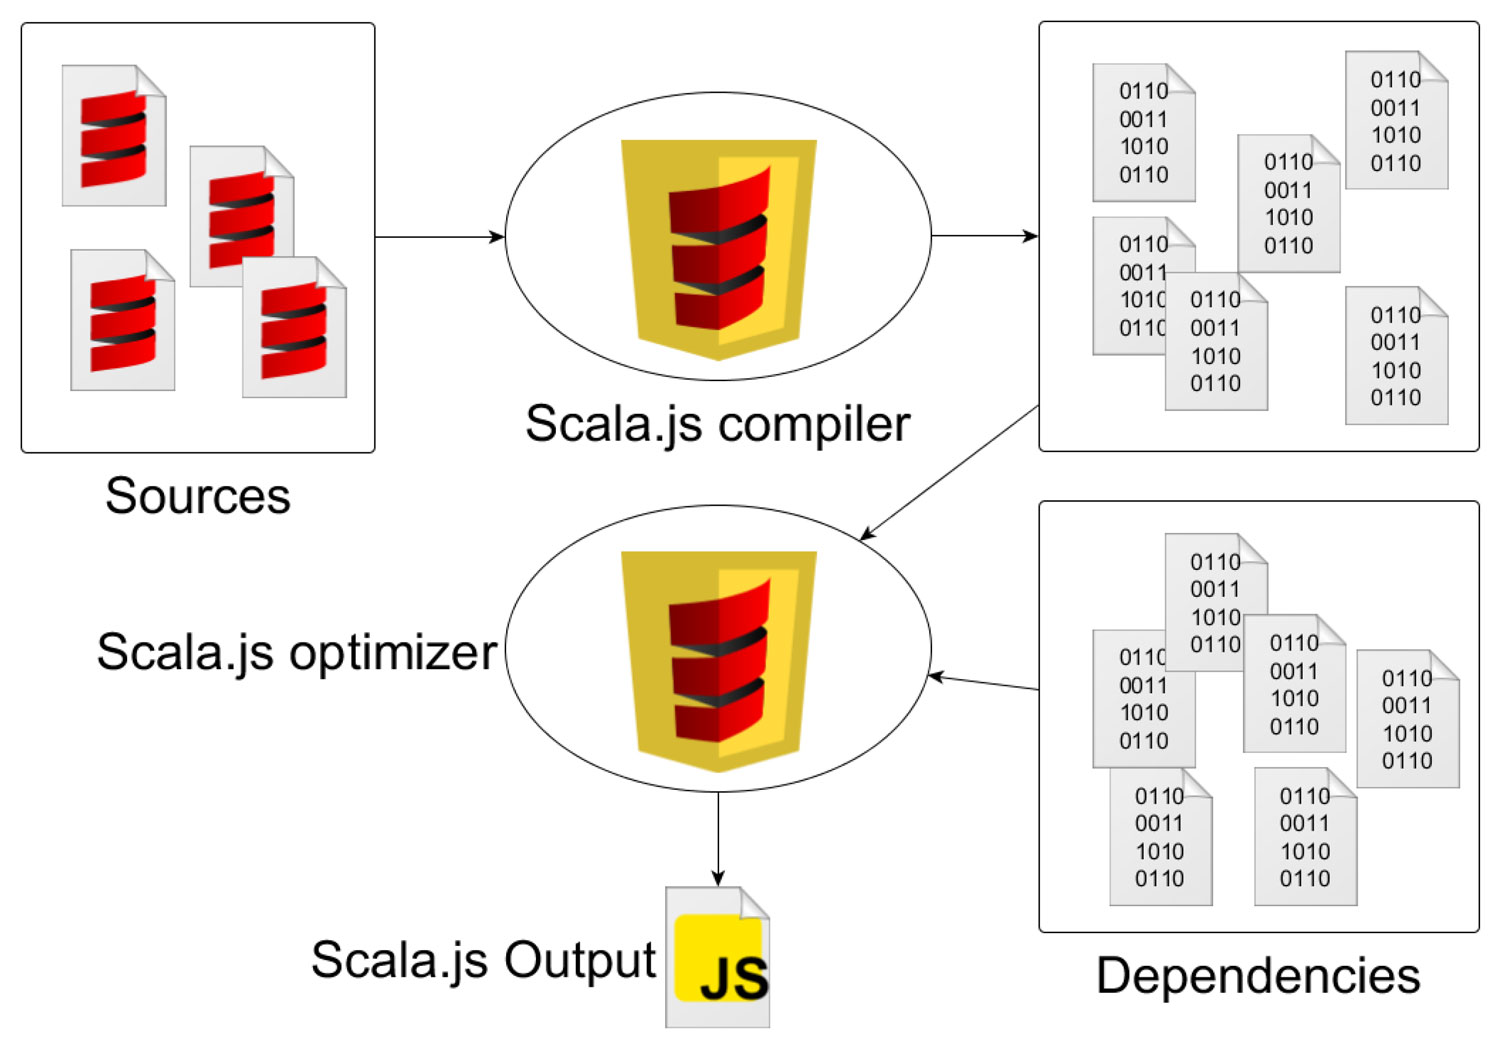
\includegraphics[
    width=0.75\textwidth
%   scale=0.5
    ]{Doeraene2014-Scalajs-p17}
    \caption{Der Scala.js-Kompilationsprozess.
    (Quelle: \cite[Folie 17]{doeraene2014.WHB})
    }
    \label{fig:sjs-compilation}
\end{figure}






% % % % % % % % % % % % % % % % % % % % % %
% % % % % % % % % % % % % % % % % % % % % %
% % % % % % % % % % % % % % % % % % % % % %





>>Projekt anlegen

%-->  \url{http://www.scala-js.org/doc/tutorial.html}

Ordnerstruktur anlegen wie folgt

TODO: Ordner-Struktur

leider nicht automatisch, es gibt (angeblich?) Plugins (???), eigenes Skript schreiben (-> Datenträger)
	- ein Weg mit IntelliJ (zu spät entdeckt): sbt-Projekt erzeugen, generiert Standard-Ordnerstruktur (inkl. leerer Java Verzeichnisse), erzeugt build.sbt, plugins.sbt und build.properties, die angepasst werden können


Scala.js-sbt-Plugin hinzufügen

Im Ordner \code{project} eine Datei \code{plugins.sbt} erzeugen:
\lstinputlisting[language=Scala, caption={Eine minimale plugins.sbt.}]{listings/setup/minimal_plugins.sbt}

Im Basisordner des Projekts eine Datei \code{build.sbt} zur Build-Definition erzeugen:
\lstinputlisting[language=Scala, caption={Eine minimale build.sbt.}]{listings/setup/minimal_build.sbt}

Hier wird das Plugin aktiviert
Name und Versionsnummer für das Projekt festgelegt
Scala-Version festlegen, muss mindestens 2.10.2 sein

mit scalaJSStage in Global := FastOptStage wird Node.js als JavaScript Runtime / Interpreter (für JS von der Kommandozeile run und test) aktiviert (statt dem langsameren Default: Rhino); Node.js muss installiert sein;

\lstinputlisting[language=Scala, caption={Eine minimale build.properties.}]{listings/setup/minimal_build.properties}
sbt-Version festlegen, muss mindestens 0.13.7 sein


strengere Compilerprüfungen durch: ...


-- build.sbt - Dependencies --

für JS-Libraries:
SalaJSKeys.jsDependencies += "org.webjars" % "jquery" % "2.1.4" / "jquery.js"

wenn es ein getyptes Interface gibt (wie für jQuery der Fall), dann genügt (webjars werden transitiv referenziert):
libraryDependencies += "be.doeraene" %%% "scalajs-jquery" % "0.8.0"

Einbindung in HTML mit einem script-Tag möglich durch:
skip in packageJSDependencies := false
FRAGE: ist das noch nötig, oder geschieht das schon automatisch?

dann in der HTML:
<script src="projectname-jsdeps.js"></script>












% % % % % % % % % % % % % % % % % % % % % %
% % % % % % % % % % % % % % % % % % % % % %
% % % % % % % % % % % % % % % % % % % % % %























\section{IDE-Support}
(http://www.scala-lang.org/news/2015/02/05/scala-js-no-longer-experimental.html)

IDE-Supports
  "With Scala.js tooling, you get syntax highlighting, code completion (even for JavaScript libraries and the DOM!), jump-to-definition, and most other features you come to expect in a Scala tooling environment" (http://www.scala-lang.org/news/2015/02/05/scala-js-no-longer-experimental.html)

  - IntelliJ IDEA  -->  https://www.jetbrains.com/idea/help/getting-started-with-scala-js.html

    Zum komfortablen Editieren und von Scala.js-Projekten
    - Code-Inspection: schlägt automatisch Scala-Code-Verbesserungen
    - Typ-Inferenz: Alt + Enter - für automatische Typ-Annotation einer Variablendefinition (Bsp. val xs = List("a", "b") wird zu val xs: List[String] = List("a", "b"))

    auch für JavaScript, HTML, CSS (in der Ultimate Edition, free für edu und open source)
      - Syntax-Highlighting
      - Code-Completion und Source-Docs zu vielen Schlüsselworten, zu JS-Standard-APIs wie DOM-API
      - jump to definition
      - intelligentes Namens-Refactoring (zumindest innerhalb einer Datei)


\section{Source Maps}

Source Maps (zum Debuggen im Browser)  -->  http://www.html5rocks.com/en/tutorials/developertools/sourcemaps/

Source Maps
  - Debugging im Browser
  http://www.html5rocks.com/en/tutorials/developertools/sourcemaps/

Dokumentation
  - Website
  - API-Docs
  - Einstieg
    - Tutorial
    - E-Book: Hands-on Scala.js
    - Scala.jsFiddle

--> Bsp. helloscalajs in Fallstudien


\section{Builds/Entwicklungszyklus und minimierter/optimierter Produktionscode}
\label{sec:compiler}

zur Link-Zeit kennt Scala.js den kompletten Code, inkl. JavaScript-Dependencies, keine Rücksichtnahme auf Laufzeit-Reflections nötig -> starke Optimierungen können vorgenommen werden
\cite[Folie 45 ff., Min. 36]{doeraene2015.SSP}
	-> Optimierungen:
		- FastOptJS
			- Dead code elimination: Code der weder im Programm aufgerufen noch mit \@JSExported exportiert wird
			- Inlining: bestimmte Methodenaufrufe werden "`ge-inlined"' -> weniger Overhead durch weniger Indirektion ((?)) (implizite Konvertierungen, Funktionen höherer Ordnung) -> schneller
			- Closure elimination: anonyme Funktionen für Funktionen höherer Ordnung wie map werden ge-inlined
		- FullOptJS -> Google Closure Compiler
			- Whitespace removal (= Entfernung von Whitespace)
			- Variablenunbemennung
			- Dead code elimination
			- Inlining
		\cite[\#HowCompilationWorks]{haoyi.HOS}

>> sbt-Konfiguration und "`Compilation und Optimization Pipeline"'

mit Google Closure Compiler  -->  https://developers.google.com/closure/compiler/
	seit August 2013 im Projekt
	- Hallo-Welt-Programm beim Prototyp noch zu 16 MB kompiliert
	- mit Google Closure Compiler Aug 2013 nur noch 900 KB

	separate (je Kompilationseinheit = Datei) und inkrementelle (nur einzelne Programmteile) Kompilierung für schnellere inkrementelle Builds
	
	komplette Scala-Library muss per dead-code-opt reduziert werden

...


-- sbt-Kommandos --

Infos hier geben tieferen Einblick scheinen aber nicht auf dem aktuellsten Stand zu sein.
\url{http://www.scala-js.org/doc/internals/compile-opt-pipeline.html}

\cite[\#TheCommandLine]{haoyi.HOS} ist hier wieder eine wertvolle und (als Mitarbeiter des Projekts) auch autorisierte Quelle -> es gibt weiter unten ein Kapitel "`The Command Line"' zum Thema.

\code{set scalaJSStage in Global := FastOptStage}

\code{set scalaJSStage in Global := FullOptStage}


\code{fastOptJS // = dev} kompiliert und optimiert (schnellerer Compiler-Lauf, größere Datei) - zur Entwicklung

\code{fullOptJS // = prod} kompiliert und optimiert (langsamerer Compiler-Lauf, aggressiver optimiert -> kleinere Datei, schnelleres JS) - zur Auslieferung

mit vorangestellter  \code{\~}, z.B. \code{\~fastOptJS}

\code{run} kompilierte Scala.js-Anwendung in einer JavaScript Laufzeit/VM (Rhino, Node.js oder PhantomJS) ausführen (main-Methode wird benötigt wie in -> Hallo-Welt)
	- läuft per default in der \textit{PreLinkStage}, verwendet Rhino
		- für DOM-API: mit \code{jsDependencies += RuntimeDOM} in der \code{build.sbt} wird die DOM-API in Rhino emuliert
	- schnellere Laufzeit (Node.js oder PhantomJS) durch \code{scalaJSStage in Global := FastOptStage} in der Build-Definition oder \code{set scalaJSStage in Global := FastOptStage} in der sbt-REPL (oder FullOptStage) aktiviert, standardmäßig Node.js
		- für DOM-API: \code{jsDependencies += RuntimeDOM} aktiviert PhantomJS (langsamer als Node.js)

\code{test} kompilierte Scala.js-Tests im \code{tests/}-Verzeichnis auf Rhino, Node.js oder PhantomJS ausführen
	- erzeugt im Verzeichnis \code{target/test-reports/} Test-Reports in XML-Form

\code{compile} kompiliert zu Scala.js Bytecode

\code{package} Scala.js-Anwendung als .jar-Datei packen (z.B. \code{hello-scalajs\_sjs0.6\_2.11-1.0.jar} mit Suffix: Scala.js-Version, Scala-Version, Projekt-Version)






Das Kommando \code{sbt fastOptJS} (bzw. \code{sbt fullOptJS}) erzeugt Dateien im Ordner
%target/scala-2.11/classes/  -- .class und .sjsir >> nicht benötigt (Output des Scala.js-Compilers: Scala/JVM-Bytecode und Scala.js-Bytecode/Zwischencode)
%target/scala-2.11/classes/  --  html << benötigt
%target/scala-2.11/  --  js << benötigt












>> hinter der Fassade / Interna

getypte Fassade vs. js.Dynamic
- Vergleich
- asInstanceOf[T]
  - Typsicherheit
  - Performance: Compiler-Optimizer kann optimieren

...






>> was ist neu
  -->  http://www.scala-js.org/news/2015/08/31/announcing-scalajs-0.6.5/
  -->  http://www.scala-js.org/doc/sjs-defined-js-classes.html





\section{Stabilität / Korrektheit / Zuverlässigkeit}

Ab Version 0.6.0 wird Rückwärtskompatibilität garantiert, und zwar sowohl bezüglich der Semantik als auch für die Standardbibliothek\footnote{Dokumentation: \url{http://www.scala-js.org/api/scalajs-library/0.6.5/\#scala.scalajs.js.package}}, (die sowohl Quellcode- als auch binärkompatibel sein wird) und mit sbt erzeugte Builds (Quellcode-kompatibel). Einzig das Format für den Scala.js-spezifischen Zwischencode (.sjsir) könnte bis zur Version 1.0.0 noch einmal geändert werden.

Die Scala Test-Suite läuft für knapp 2000 Tests, die das erwartungsgemäße Kompilieren beziehungsweise Nicht-Kompilieren prüfen, zu 99\% erfolgreich durch. Von über 1000 Tests, die die korrekte Ausführung überprüfen, sind nur 51 \% erfolgreich \cite[Folie 36, Min. 35]{doeraene2014.WHB}. Bei den wenigsten der Fehlschläge handelt es sich laut Doeraene allerdings tatsächlich um Bugs. Der Grund hierfür liegt darin, dass Scala.js bestimmte Spracheigenschaften wie Laufzeit-Reflections und die Java Collections nicht unterstützt \cite[S. 7]{doeraene2013.TDI}. Zusätzlich gibt es eine eigene Test-Suite mit über 400 Tests \cite[Folie 36, Min. 35]{doeraene2014.WHB}.




\section{Ökosystem: Libraries und Tools}\label{sec:sjs-libs}

>> verwendete/ausprobierte/untersuchte Libraries (2)

\subsubsection{Scala-js-dom}

- statische Typen für die DOM-API, Erweiterungen

-> doeraene TDI S. 8 links oben:
	von Li Haoy, durch automatische Übersetzung von TypeScript-Typen

http://scala-js.github.io/scala-js-dom/
scalajs.dom.ext.Color

\subsubsection{(scala-js-jquery)}

- statische Typen für jQuery. (Alternativ gibt es die Bibliothek \code{jquery-facade}, die aber nicht ausprobiert wurde.))

\subsubsection{ScalaTags}

- cross-kompilierende HTML-Templating-Library (mehr Typsicherheit für Tags)

Motivation
%  -->  http://lihaoyi.github.io/scalatags/#WhyScalatags
%  -->  http://lihaoyi.github.io/scalatags/#PriorWork



mit \scala{TypedTag[html.Element].render} wird eine DOM-Tree-Node erzeugt
  val foo = div("`foo"').render
  assert(foo.textContent == "foo")
  foo.text
  assert(foo.textContent == "foo")
%  --> http://lihaoyi.github.io/scalatags/#UsingtheDOM

erlaubt direkten Zugriff auf referenzierte Elemente ohne Suche im DOM mit DOM-Selektoren (mit document.getElementById(...) bzw. jQuery)
%  -->  http://lihaoyi.github.io/scalatags/#UseCases

ScalaTags: importe / Bundles - schwer zu verstehen, am einfachsten JsDom.all\_, aber dann clutter im Namespace

CSS/Style - wenn nötig können Attribute und Styles in Variablen gemerkt werden; auf diese Weise können auch eigene Attribute festgelegt werden, die Scalatags nicht kennt:
%  val dataAppKey = "data-app-key".attr
%  val customBackgroundStyle = "background-color".style
%  div(
%    dataAppKey:="YOUR_APP_KEY",
%    customBackgroundStyle:="red"
%  )

(CSS mit Vererbung
%  -->  http://lihaoyi.github.io/scalatags/#CSSStylesheets)

Vertiefung
%  -->  http://lihaoyi.github.io/scalatags/#Internals


\subsubsection{utest}

- minimale cross-kompilierende Test-Library

mögliche Macros:
\begin{lstlisting}[language=Scala]
object MyTest extends TestSuite {
  override def tests = TestSuite{
    "foo" - {
      assert(1 + 1 == 2)
      assertMatch(List(1, 2, 3)){case 1 :: _ => }
      intercept[NoSuchElementException](Nil.head)
      compileError("val x: Int = 1.2")
    }
  }
}
\end{lstlisting}

assert und intercept wie in ScalaTest


asynchrone Tests mit Futures möglich, aber nicht erforscht

Die bekannten Test-Bibliotheken ScalaTest und Specs2 können nicht verwendet werden, da sie zu stark von Java-Spezifika abhängen, um nach Scala.js portiert werden zu können\cite[\#OtherTestingLibraries]{haoyi.HOS}.


\subsubsection{(uPickle)}

- cross-kompilierende Library zur Serialisierung)


\subsubsection{autowire}

- cross-kompilierende Library für statisch getypte Ajax-Aufrufe und RPCs

\subsubsection{(spray)}

- Sammlung von Libraries zur Entwicklung von REST/HTTP-basierten Webservices auf der Basis von Akka; beinhaltet spray-can, einen schnellen HTTP-Server)

\subsubsection{(Scala.Rx)}

- cross-kompilierende Change-Propagation-Library ("Änderungsausbreitung"))

\subsubsection{Scala-Async}

- Scala-Library zur einfacheren Handhabung von Asynchronität; funktioniert mit Scala.js -->  http://docs.scala-lang.org/sips/pending/async.html

\subsubsection{Scala.js workbench}

- sbt-Plugin zum automatischen Live-Neuladen des Browsers


Check: alle Infos up-to-date?
-->  http://www.scala-js.org/news/2015/02/05/announcing-scalajs-0.6.0/
-->  http://www.scala-js.org/news/2015/08/31/announcing-scalajs-0.6.5/





% % % % % % % % % % % % % % % % % % % % % % % % % % % % % % % %
\chapter{Methodik}

>>Ziele

Verwendungsweise(?) - wie funktioniert es in der Anwendung
Konfiguration
	wie?
	Aufwand
Performance
	Build: Compiler, Tests
Wartbarkeit, Entwicklerfreundlichkeit
	Debugging-Qualitäten
	Code-Qualität
	Entwicklungsgeschwindigkeit (?)
	Dokumentation
Nützlichkeit: Umsetzbarkeit von Anforderungen der Web-Entwicklung
	DOM
	Events
	Canvas
	AJAX

\section{Kriterien der Evaluierung}

%\subsection{anwenderbezogen}
%
%Anforderungen an interaktive Webseiten
%- schnell laden
%- Interaktionen sollen sich schnell anfühlen
%- sollen regelmäßig weiterentwickelt werden
%
%\subsubsection{Korrektheit}
%\subsubsection{Performance}
%\paragraph{Seitenladezeit}
%\paragraph{Speicherbedarf/"`Page weight"'}
%\paragraph{Ausführungszeit von Funktionen}
%\paragraph{(Speicherbelastung)}
%\paragraph{(CPU-Belastung)}
%
%\subsection{entwicklerbezogen}
%
%TODO Antworten ins Kapitel "`Auswertung ..."'
%
%Anforderungen an Entwicklungswerkzeuge
%- siehe \url{http://www.scala-js.org/doc/cookbook/}
%- ...
%- Kompatibilität:
%  - siehe Doeraene: SJS. What has it become, 19:00  -->  \url{https://www.parleys.com/tutorial/scala-js-what-has-become-how-used-wild}
%Dokumentation:
%	- offizielle Referenzseite
%	  - API-Doku - vollständig (?) aber knapp
%	  - Tutorial
%	- Hands-on Scala
%???:
%	- Scala-Js-Fiddle  -->  http://www.scala-js-fiddle.com/
%Tests:
%	- utest - für JVM und JS
%
%\subsection{Code-Qualität}
%\paragraph{Typsicherheit}
%\paragraph{LOC (Lines of Code)}
%\paragraph{Komplexität}
%\paragraph{Lesbarkeit/Verständlichkeit}
%\paragraph{"`Debugbarkeit"'/Wartbarkeit, Erweiterbarkeit, Wiederverwendbarkeit}
%
%\subsection{JavaScript-Interoperabilität}
%
%\subsection{Konfiguarationsaufwand}
%
%\subsection{alles umsetzbar? Grenzen? alle Anwendungsfälle abgedeckt?}
%
%\subsection{Dokumentation}
%
%\subsection{Unterstützung durch Tools, Entwicklungsgeschwindigkeit}
%
%\subsection{Support/Fachforen etc.}
%
%
%\section{Gewählte Testverfahren und -techniken}
%
%\subsection{m01 - Vergleichs-Implementierung in reinem JavaScript/HTML}
%\subsection{m02 - HTML-Validierung}
%\subsection{m03 - Unit-Tests mit Jasmine (für Vergleich Scala.js/JavaScript)}
%\subsection{m04 - Unit-Tests mit utest}
%\subsection{m05 - Seitenladezeit messen mit Webpagetest und YSlow}
%\subsection{m06 - Profiling mit Chrome Developer Tools}
%\subsection{m07 - Benchmarks mit JSLitmus und Benchmark.js}
%\subsection{m08 - Halstead-Metrik}
%\subsection{m09 - Anzahl zusätzlicher Library-Dependencies}
%\subsection{m10 - empirische/experimentell}

\section{Vorgehensweise bei der Untersuchung}

%Matrix - welche Methode für welche Kriterien


% % % % % % % % % % % % % % % % % % % % % % % % % % % % % % % %
\chapter{Projekt-Setup, Installation}

%TODO (Abweichungen ggf. separat bei der jeweiligen Anwendung)

Die nachfolgende Anleitung bezieht sich auf die Installation auf einem Windows-8.1-Rechner. Auf anderen Plattform können einzelne Schritte im Detail abweichen.

Um die Installation erfolgreich durchführen zu können ist eine gute Internetverbindung erforderlich, da die einige Bibliotheken heruntergeladen müssen. Außerdem wird ein aktueller Browser benötigt. Für volle \textit{Sourcemaps}-Unterstützung in der Browser-Konsole empfiehlt sich hier Google Chrome\footnote{\url{https://www.google.de/chrome/browser/desktop/}}.

Die folgende Software wird benötigt:

\begin{itemize}
	\item Java Development Kit (JDK) 8\footnote{ggf. genügt auch ein JRE}  --  \url{www.oracle.com/technetwork/java/javase/}
	\item Scala  --  \url{http://www.scala-lang.org/}
	\item sbt  --  \url{http://www.scala-sbt.org/}
	\item git  --  \url{https://git-scm.com/}
	\item Node.js  --  \url{https://nodejs.org/en/}
	\item PhantomJS  --  \url{http://phantomjs.org/}
\end{itemize}

Alle benötigten Programme sind auf dem beigefügten Datenträger enthalten, lassen sich alternativ auch unter der angegebenen Adresse beim Hersteller herunterladen. Bei Bedarf finden sich dort auch Installationsanleitungen, die allerdings nicht benötigt werden sollten. Für Windows existieren ausführbare Installationsprogramme, die selbsterklärend sind. PhantomJS muss nicht installiert werden; hier genügt es, den Inhalt der .zip-Datei ins gewünschte Programmverzeichnis zu entpacken.

Für alle Programme mit Ausnahme von git ist es unter Windows nötig, dem System den Installationspfad bekannt zu machen. Dies geschieht durch Setzen einer entsprechenden Umgebungsvariablen. Dazu muss der "`System"'-Dialog geöffnet werden, zum Beispiel durch die Tastenkombination \code{Windows-Taste + x}. Hier "`Erweiterte Systemeigenschaften"' mit Administrator-Rechten öffnen und die folgende Frage, ob Änderungen am System zugelassen werden sollen mit "`Ja"' bestätigen. Nun den Knopf "`Umgebungsvariablen"' betätigen, die Variable "`Path"' auswählen und auf "`Bearbeiten..."' klicken. Hier muss nun der Pfad der die ausführbare Datei für das entsprechende Programm enthält angegeben werden. Das ist für alle benötigten Programme mit Ausnahme von Node.js der Ordner \code{bin} im jeweiligen Programmverzeichnis. Dieser Pfad muss nun mit getrennt durch ein vorangestelltes Semikolon hinten an den ursprünglichen Wert angehängt werden. Für Java muss zum Beispiel \code{;C:\\Program Files\\Java\\jdk1.8.0\_51\\bin} angehängt werden.

Als Terminal wurde die git-bash vewendet, die in der Windows-Distribution von git enthalten ist. Alternativ kann auch die bash-Emulation von cygwin verwendet werden. Wenn IntelliJ IDEA verwendet wird, kann auch direkt von dort aus mit dem Terminal gearbeitet werden\footnote{\url{https://www.jetbrains.com/idea/help/working-with-embedded-local-terminal.html}}.

Scala.js muss nicht installiert werden sondern wird durch per Build-Definition als sbt-Plugin gestartet.

Für die bequemere Navigation im Projekt bietet sich der Einsatz IDE an. Infrage kommen:

\begin{description}
	\item[IntelliJ IDEA] liefert am meisten Komfort, unterstützt sbt schon am besten und ist deshalb klar die erste Wahl. Scala wird bei der aktuellen Version von Hause aus unterstützt, ältere Versionen lassen sich mit einem Plugin nachrüsten.
	\item[Scala IDE / Eclipse] funktioniert recht gut. Allerdings fehlt sbt-Unterstützung.
	\item[Netbeans] kommt ebenfalls in Betracht, wurde allerdings nicht erprobt. Hierfür existiert ein Scala-Plugin.
\end{description}


(Scala IDE oder/und  installieren; IntelliJ unterstütz Scala, für ältere Versionen Scala Plugin installieren)
(Google Chrome installieren - hat Sourcemaps-Unterstützung)



\section{IDE-Integration}

== in IntelliJ importieren ==

momentan komfortabler, sowohl Import als auch IDE-Support
	- bessere Integration mit sbt

- 1. IntelliJ > File > New > Project from Existing Sources...
- 2. Ordner auswählen
- 3. OK
- 4. Import project from external model > SBT
- 5. Next
- 6. check: Download sources and docs - wenn versucht werden soll, die Quellen der Library-Dependencies herunterzuladen
- 7. Finish

File > New > Project from Existing Sources...
alternativ: Welcome > Import Project
Select File or Directory to Import -- Projektordner (der build.sbt enthält) auswählen -- Ok
Import Project -- "Import project from external model" auswählen -- SBT auswählen -- Next
Import Project -- "Download sources and docs" auswählen -- Finish

Es ist auch möglich, mit sbt ein eine 


\begin{figure}[!h]
    \centering
    
\includegraphics[
    width=0.25\linewidth
%   scale=0.5
    ]{tux}
    \caption{Eine Beispielabbildung.
    (Quelle: \cite{aab.FBB})
    }
    \label{fig:a_picture_of_tux}
\end{figure}

Änderungen an sbt-Konfigurationsdateien werden von IntelliJ erkannt; das Programm schlägt einen "Refresh" vor, der ausgeführt werden sollte
erkennt sbt-Dateien und unterstützt automatische Vervollständigung


== in Scala IDE importieren ==

Plugin: sbteclipse\footnote{\url{https://github.com/typesafehub/sbteclipse}}

dieses erzeugt ein Eclipse-Projekt

in project/plugins.sbt hinzufügen:
\begin{lstlisting}[language=Scala, style=snippet]
addSbtPlugin("com.typesafe.sbteclipse" % "sbteclipse-plugin" % "4.0.0")
\end{lstlisting}

wenn sbteclipse versuchen soll, die Quellen der Library-Dependencies herunterzuladen - in build.sbt hinzufügen:

\begin{lstlisting}[language=Scala, style=snippet]
EclipseKeys.withSource := true
\end{lstlisting}



- 1. run:
  sbt eclipse  --  .project und .classpath erzeugt, kann nun importiert werden
- 2. Scala IDE > File > Import > Existing Projects into Workspace
- 3. Ordner auswählen
- 4. Finish


Eclipse erzeugt standardmäßig einen Verzeichnis bin im Projektwurzelverzeichnis, als Zielordner des Compilers ...

nach Änderungen an sbt-Konfigurationsdateien ist es nötig, erneut \code{sbt eclipse} auszuführen und das Projekt in Eclipse im Package Explorer zu aktualisieren.






\section{Konfiguration von Node.js (und Karma?), source-map-support}

Node.js ...

Damit Stacktraces richtig aufgelöst werden sollte \textit{source-map-support}\footnote{\url{https://www.npmjs.com/package/source-map-support}} im Projekt installiert werden mit:

\begin{lstlisting}[style=snippet]
npm install source-map-support
\end{lstlisting}

Die Dateien des Plugins werden im Projektverzeichnis in einem frisch erzeugten Ordner \code{node\_modules} abgelegt.

Es ist auch möglich, das Projekt als Node.js-Projekt zu initialisieren. Das hat den Vorteil, dass man sich die benötigte Dependency in einer Konfigurationsdatei merken kann.

\begin{lstlisting}[style=snippet]
npm -y init
npm install source-map-support --save-dev
\end{lstlisting}

Künftig kann der \code{node\_modules}-Ordner bedenkenlos gelöscht werden. Ein einfacher Aufruf von \code{npm install} genügt um alle benötigten Node.js-Pakete zu laden.


\section{Installation und Start von Anwendung und Tests}

- Sourcen von Datenträger oder github(?) (-> git client), hierzu genügt der Aufruf git clone <repo> vom Terminal im gewünschten Verzeichnis
- Kommandos zum kompilieren --> sbt-Abschnitt - hierher???
- Readme für jedes Projekt mit ggf. abweichenden spezifischen Anweisungen zum Start der jeweiligen Anwendung


% % % % % % % % % % % % % % % % % % % % % % % % % % % % % % % %
\chapter{Fallstudien (20)}


bei den Eingangsbeispielen gestützt auf
-->  Scala.js-Tutorial

wichtige Quelle
-->  Hands-on Scala.js

%TODO Liste der Beispielprojekte, verlinkt auf GitHub
TODO Liste der Beispielprojekte, verlinkt auf GitHub


% % % % % % % % % % % % % % % % % % % % % % % % % % % % % % % %
\section{Ein Minimalbeispiel: Hello Scala.js}

%TODO Hinweis: lose orientiert an  -->  http://www.scala-js.org/doc/tutorial.html

\subsection{Ziel der Untersuchung}

Ein minimales Setup in Form eines klassischen Hallo-Welt-Programms sollte zum Laufen gebracht werden. Anhand dieses Minimalbeispiels sollten dann bestimmte Grundbedingungen der Entwicklung mit Scala.js untersucht werden. Neben der Konfiguration selbst sollte als wichtiger Faktor für die alltägliche Entwicklungsarbeit die Zeit ermittelt werden, die für einen Build-Lauf benötigt wird. Auch die Größe der für die Auslieferung relevanten Kompilate sollte betrachtet werden, schließlich besteht ein unmittelbarer Zusammenhang zwischen der Größe der zu ladenden Datenmenge und der Ladezeit im Browser, weshalb sie eine wichtige Grundbedingung für die Zufriedenheit der Benutzer ist.

Anhand einer erweiterten Fassung des Minimalbeispiel sollten Benutzerinteraktion und der Einsatz von jQuery ausprobiert und die Testbarkeit von Oberflächen-Elementen geklärt werden. Außerdem sollte die Sourcemap-Unterstützung erprobt werden.

document.createElement("div")
\subsection{Kriterien}

\begin{enumerate}
	\item Konfigurationsaufwand
	\item Performance
	\begin{enumerate}
		\item Compiler-Geschwindigkeit
		\item Größe der Kompilate
	\end{enumerate}
	\item Wartbarkeit
		\begin{enumerate}
			\item Debugging-Qualitäten
			\item Testbarkeit
		\end{enumerate}
\end{enumerate}

\subsection{Kurzbeschreibung des Beispielprogramms}

Das minimale Programm erzeugt die Ausgabe "`Hello world!"' in der Konsole des Browsers, wenn die entsprechende Webseite geöffnet wird. Der Aufruf \code{sbt run} erzeugt die gleiche Ausgabe in der sbt-REPL.

Der benötigte Scala-Code ist überschaubar, wie Listing \ref{code:hello.scala} zeigt.

\lstinputlisting[language=Scala, caption={Scala.js-Code für ein Hallo-Welt-Programm.}, label={code:hello.scala}]{listings/01hello-scalajs/HelloApp.scala}

\scala{HelloApp} erbt vom Trait \scala{JSApp}, der eine \scala{main}-Methode mit Rückgabetyp \scala{Unit} verlangt. Dadurch kann die \scala{HelloApp} mit ihrer \scala{main}-Methode nun in JavaScript unter ihrem voll qualifizierten Namen verwendet werden. Die Methode \scala{println} benutzt die Standardausgabe. Wenn das Programm in der sbt-REPL ausgeführt wird ist es die Konsole dort, im Browser wird die Browser-Konsole verwendet.

Dieses Programm lässt sich bereits auf der sbt-Konsole ausführen (Listing \ref{code:run-hello}).

\begin{lstlisting}[caption={Lauf des Hallo-Welt-Programms in der sbt-REPL.}, label={code:run-hello}]
$ sbt
> run
[...]
[info] Updating {[...]/hello-scalajs/}hello-scalajs...
[info] Resolving [...] ...
[info] Done updating.
[info] Compiling 1 Scala source to [...]\hello-scalajs\target\scala-2.11\classes...
[info] Fast optimizing [...]\hello-scalajs\target\scala-2.11\hello-scalajs-fastopt.js
[info] Running hello.HelloApp
Hello world!
[success] [...]
\end{lstlisting}

Damit das kleine Programm im Browser ausgeführt werden kann, muß es in eine HTML-Datei eingebunden werden, wie in Listing \ref{code:hello.html}.

\lstinputlisting[language=HTML5, caption={HTML-Code zur Einbindung der Scala.js-Datei in eine Website.}, label={code:hello.html}]{listings/01hello-scalajs/index-dev.html}

Hierbei empfehlen sich zwei getrennte HTML-Dateien, eine zur Entwicklung und eine für das fertige Produkt, in der die jeweils passenden JavaScript-Dateien zu verwenden sind. Wie in Abschnitt~\ref{sec:compiler} beschrieben, erzeugt der Scala.js-Compiler, je nach Task, \code{fastOptJS} oder \code{fullOptJS}, unterschiedliche JavaScript-Dateien, die anhand ihres Suffix, \code{-fastopt.js} beziehungsweise \code{-opt.js}, auseinandergehalten werden können. Die Pflege von zwei nahezu identischen HTML-Dokumenten mag etwas ärgerlich scheinen. Andererseits besteht ihr Hauptzweck in der unterschiedlichen Konfiguration für Entwicklung oder Produktion.

Das erweiterte Minimalbeispiel reagiert auf Betätigung eines Buttons hin mit einer Text-Ausgabe sowohl auf die Browser-Konsole als auch in die Webseite.

\begin{figure}[!h]
    \centering
    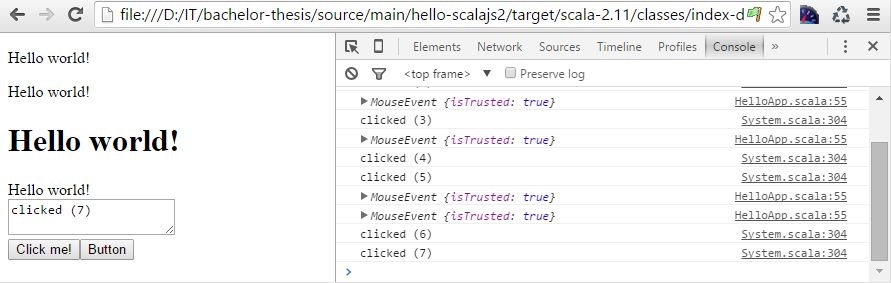
\includegraphics[
    width=1.0\textwidth
%   scale=0.5
    ]{hello-scalajs/hello2}
    \caption{Erweitertes Minimalbeispiel mit Benutzerinteraktion.
    (Quelle: eigene Anfertigung)
    }
    \label{fig:hello2}
\end{figure}

\subsection{Ergebnisse der Untersuchung und Bewertung}

\subsubsection{Konfigurationsaufwand}

Im direkten Vergleich mit einem Programm in reinem JavaScript und HTML (Listing \ref{code:hello-js.html}):

\lstinputlisting[language=HTML5, caption={HTML-Code mit eingebettetem JavaScript für ein Hallo-Welt-Programm.}, label={code:hello-js.html}]{listings/01hello-scalajs/hello-js-index.html}

ist der Aufwand, der für ein Scala.js-Projekt mit gleicher Funktionalität betrieben werden muss deutlich größer. Was sich dort auf eine einzige Datei mit wenigen Zeilen Code beschränkt, benötigt hier Build-Definitionen, Plugins und eine ganze Projektstruktur. Andererseits schlägt sich der Gewinn, der sich daraus ergibt, typsicher in Scala für die Oberfläche zu programmieren, bei einem so trivialen Beispiel noch nicht nieder.

Die Einbindung von \code{scala-js-jquery} unkompliziert. Dau muss lediglich
\begin{lstlisting}[style=snippet]
libraryDependencies += "be.doeraene" %%% "scalajs-jquery" % "0.8.0"
\end{lstlisting}
in der \code{buil.sbt} hinzugefügt werden.

Etwas schwieriger war aber, zu verstehen wie sich hier und generell minifizierte Versionen für die im \code{target/}-Ordner erzeugten JavaScript-Dependencies erzwingen lassen (siehe (???)).

Für Tests wurde \code{uTest} verwendet und ensprechend den \code{libraryDependencies} hinzugefügt. Um dem DOM für Tests verwenden zu können, muss wie in Kapitel (sbt-Integration ???) beschrieben, der Eintrag
\begin{lstlisting}[style=snippet]
jsDependencies in Test += RuntimeDOM
\end{lstlisting}
in der Build-Definition ergänzt werden.

Um Sourcemaps-Unterstützung im Browser zu bekommen, muss eine nicht allzu aufwendige Installation vorgenommen werden, wie in ((???)) beschrieben.

\subsubsection{Performance}

Hier wurde die Geschwindigkeit des Build-Laufs und die Größe der Kompilate untersucht.

Es wurde Windows 8.1 Pro auf einem System mit 64-Bit Intel Core i7-3517U Prozessor mit einem Takt von 1,9 GHz, 4 GB RAM und einem SSD-Laufwerk verwendet.

Die Ergebnisse der Untersuchung sind in den Tabellen \ref{table:compiler-performance1} und \ref{table:compiler-performance2} dargestellt.

\medskip

\begin{table}[!h]
\begin{tabular}{|l|r|r|r|r|r|r||r|r|r|r|}
\hline           & t1   & t2   & t3   & t4   & tc            & tn    & s0             & s1     & sm    & sd    \\ 
\hline fullOptJS & 10 s &  4 s &  3 s &  3 s &          2 s  & 0-1 s & \textbf{20 kB} &  77 kB & 57 kB &  0 kB \\ 
\hline fastOptJS &  7 s &  3 s &  3 s &  2 s &  \textbf{2 s} & 0-1 s &        101 kB  & 193 kB & 92 kB &  0 kB \\ 
\hline 
\end{tabular} 
\caption{Build-Performance für ein minimales Hallo-Welt-Programm.}
\label{table:compiler-performance1}
\end{table}

\medskip

\begin{table}[!h]
\begin{tabular}{|l|r|r|r|r|r|r||r|r|r|r|}
\hline           & t1   & t2   & t3   & t4   & tc            & tn    & s0             & s1     & sm     & sd     \\ 
\hline fullOptJS & 15 s &  7 s &  5 s &  5 s &          4 s  & 0-1 s & \textbf{57 kB} & 230 kB & 173 kB &   0 kB \\ 
\hline fastOptJS & 11 s &  5 s &  4 s &  4 s &  \textbf{3 s} & 0-1 s &        277 kB  & 520 kB & 243 kB &   0 kB \\ 
\hline test      & 35 s & 24 s & 24 s & 22 s &         19 s  &  16 s &        1,6 MB  & 2,8 MB & 1,2 MB & 241 kB \\ 
\hline 
\end{tabular} 
\caption{Build-Performance für ein leicht erweitertes Hallo-Welt-Programm mit Tests.}
\label{table:compiler-performance2}
\end{table}

\medskip

Die verwendeten Abkürzungen sind in der Legende \ref{table:compiler-performance-legend} aufgeschlüsselt.

\medskip

\begin{table}[!h]
\begin{tabular}{|l|l|}
\hline t1 & Dauer des 1. Compilerlaufs (target-Ordner existiert noch nicht) \\ 
\hline t2 & Dauer des 2. Compilerlauf nach einem \code{clean} \\ 
\hline t3 & Dauer des 3. Compilerlauf nach einem \code{clean} \\ 
\hline t4 & Dauer des 4. Compilerlauf nach einem \code{clean} \\ 
\hline tc & Dauer ab 2. Compilerlauf mit Code-Änderungen ohne \code{clean} \\ 
\hline tn & Dauer ab 2. Compilerlauf ohne Code-Änderungen ohne \code{clean} \\ 
\hline s0 & Größe der erzeugten Dateien ohne Sourcemaps \\ 
\hline s1 & Größe der erzeugten Dateien mit Sourcemaps \\ 
\hline sm & Größe der erzeugten Sourcemaps-Datei \\ 
\hline sd & Größe der erzeugten Datei, die die JavaScript-Dependencies enthält \\ 
\hline 
\end{tabular} 
\caption{Legende zu \ref{table:compiler-performance1} und \ref{table:compiler-performance2}.}
\label{table:compiler-performance-legend}
\end{table}

\medskip

Für die ermittelten Dateigrößen wurde der erzeugte Bytecode (die \code{.class}- und \code{.sjsir}-Dateien) nicht mitgerechnet.

\code{test} wurde immer in der FastOpt-Stage mit PhantomJS verwendet. Zwischen den Testläufen wurde nie \code{clean} aufgerufen. Für den ersten Testlauf existierte kein target-Ordner beziehungsweise dieser wurde zuvor gelöscht.

Es wird deutlich, dass sich der Compiler ab dem zweiten Lauf "`stabilisiert"' und selbst nach einem \textbf{clean} deutlich schneller fertig ist als beim ersten Lauf. Der für den Entwicklungsalltag häufiste Fall dürfte wohl ein Build nach Code-Änderungen ohne \textbf{clean} sein. Dafür sind 3 Sekunden eine vertretbare Zeit. Bei einem weniger trivialen Beispiel mit mehr Code wachsen diese Zeiten, bleiben aber den Erfahrungen im Laufe dieser Arbeit nach in der Regel unter 10 Sekunden (? TODO: CHECK --> clientserver oder stringanalyzer) und damit in einem vertretbaren Rahmen.

Es ist auch zu erkennen, dass Testläufe, selbst ohne Code-Änderungen nicht besonders schnell sind. In den insgesamt 7 Tests werden 25 Assertions verwendet.\footnote{Im Code stehen 13 Assertions, davon werden 3 jeweils in einer Schleife 5-mal aufgerufen.} Hier darf gemutmaßt werden, ob dabei auch die Ausführungsgeschwindigkeit von PhantomJS eine Rolle spielt. Schnellere Testläufe wären hier in jedem Fall wünschenswert. Andererseits fallen etwas langsamere Tests weniger ins Gewicht, wenn man im kontinuierlichen Modus arbeitet (zu erreichen mit dem Kommando \code{\~test}).

Die Größe der Kompilate übertrifft reines HTML/JavaScript (187 Bytes) um einen Faktor von etwa 100. Andererseits ist dieser Vergleich nicht ganz fair. Ein Großer Teil der von Scala.js generierten JavaScript-Datei ist die Scala-Standardbibliothek.
Der Optimierer und der Google Closure Compiler reduzieren die Code-Menge (durch Techniken wie \textit{dead code elimination} oder die aggressive Verkürzung von Variablennamen) schon sehr stark. Die Größe von Dateien voll optimiertem Scala.js-generierten JavaScript-Dateien wird deshalb mit wachsender Code-Basis des eigenen Software-Projekts nicht etwa proportional, sondern langsamer anwachsen. Li Haoyi verweist zum Beispiel auf ein eigenes Projekt mit einem Umfang von ca. 2000 Zeilen Code, welches voll optimiert noch 288 kB groß ist. (TODO! -> eigenes client-server-Bsp.) Das Problem wird weiter relativiert durch die Tatsache, dass die meisten Server ihre Daten gzip-komprimiert übertragen, was laut Haoyi die Datenlast auf etwa ein Zehntel verkleinert.\cite[\#BlobSize]{haoyi.HOS}

\subsubsection{Debugging-Qualitäten}

%TODO$$$$$$$$$$$$$$$$$$$$$$$$$$$$$$$

Eine einfache Art des Debuggings besteht im Schreiben in die Konsole. Nun funktioniert es mit Scala.js hervorragend, mit \scala{println} einfache Ausgaben auf die Browser-Konsole zu machen. Möchte man allerdings den Inhalt von Objekten inspizieren, so genügt das häufig nicht. 

Angenommen wir, haben eine Klasse \scala{class A(foo: Int, bar: String)} von der wir eine Instanz \scala{foo(123, "baz")} erzeugen. \scala{println(foo)} --> --> --> \scala{println(foo.toString)}
Da verwendet \scala{toString}, wenn nicht überschrieben -> manchmal \js{[object Object]}
aber mit dom.console.log kann man ohne toString-Methode direkt das Objekt inspizieren -> \js{Object {foo: 123, bar: "baz"}}

Der Einsatz von Sourcemaps erhöht den Komfort beim Debugging in der Browser-Konsole\footnote{Erprobt wurde hierbei Chrome.} erheblich. Wie der Vergleich in den Abbildungen \ref{fig:no-sourcemaps} und \ref{fig:sourcemaps} zeigt, macht es selbst beim nicht-minifizierten Entwicklungs-Code einen großen Unterschied, ob man zur originalen Scala-Code springen kann, oder ob man gezwungen ist, compilergeneriertes JavaScript zu verstehen. Selbst im \code{FullOpt}-Modus funktioniert übrigens die Auflösung der Referenzen zum Scala-Code.
\url{http://www.html5rocks.com/en/tutorials/developertools/sourcemaps/}
	- sinvoller Stacktrace in der Browserkonsole durch ...
	
	(siehe dazu Abb. \ref{fig:no-sourcemaps} und \ref{fig:sourcemaps})

\begin{figure}[!h]
	\centering
	\subfloat[][]{
		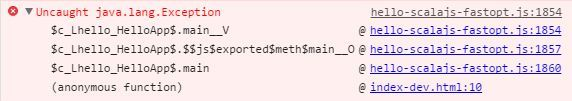
\includegraphics[width=0.66\textwidth]{sourcemaps1-dumb-stacktrace}
		\label{fig:sourcemaps1}
	}
	\subfloat[][]{
		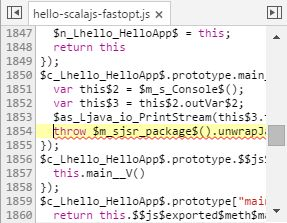
\includegraphics[width=0.33\textwidth]{sourcemaps2-cryptic-code}
		\label{fig:sourcemaps2}
	}
	\caption{Ohne Sourcemaps: Wenig aussagekräftiger Stacktrace \protect\subref{fig:sourcemaps1}, navigierbar zu schwer verständlichem, generierten JavaScript-Code \protect\subref{fig:sourcemaps2}. (Quelle: eigene Anfertigung)}
	\label{fig:no-sourcemaps}
\end{figure}

\begin{figure}[!h]
	\centering
	\subfloat[][]{
		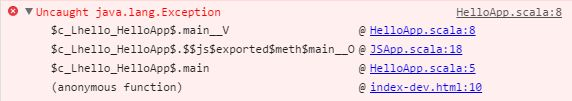
\includegraphics[width=0.66\textwidth]{sourcemaps3-smart-stacktrace}
		\label{fig:sourcemaps3}
	}
	\subfloat[][]{
		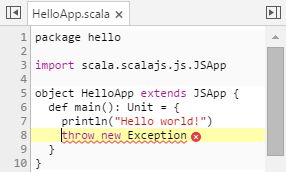
\includegraphics[width=0.33\textwidth]{sourcemaps4-legible-code}
		\label{fig:sourcemaps4}
	}
	\caption{Unterstützung durch Sourcemaps: Diagnosestärkerer Stacktrace \protect\subref{fig:sourcemaps3}, navigierbar zu verständlichem Scala-Code \protect\subref{fig:sourcemaps4}. (Quelle: eigene Anfertigung)}
	\label{fig:sourcemaps}
\end{figure}


\subsubsection{Testbarkeit}

Mit der verwendeten Test-Biliothek uTest lassen sich Tests formulieren, um zu prüfen, dass HTML-Elemente wie erwartet existieren oder dass Buttons erwartungsgemäß reagieren. Allerdings ist es hierfür nötig, die betreffenden HTML-Elemente mit eindeutigen IDs zu versehen, was einen zusätzlichen Overhead darstellt. Für eine leichtere Selektion von HTML-Elementen in Tests erweist sich darüber hinaus der Einsatz von jQuery als nützlich. Was hier fehlt, ist die Möglichkeit, wie im JavaScript-Test-Framework Jasmine, mithilfe sogenannter \textit{Spies} prüfen zu können, ob und mit welchen Argumenten eine Methode aufgerufen wurde.\footnote{\url{http://jasmine.github.io/2.0/introduction.html\#section-Spies}} Für Scala.js existiert zwar ein Wrapper für Jasmine. In einer Ankündigung auf der offiziellen Scala.js-Webseite\cite{scalajs.ASJ} wird aber explizit von dessen Verwendung abgeraten. Grundsätzlich lässt sich mit uTest gut arbeiten, allerdings erhält man beim Fehlschlagen von Tests häufig einen sehr langen Stacktrace. Für einen größeren Komfort wäre hier für die Zukunft ein IDE-Plugin mit navigierbarem Stacktrace wünschenswert.





% % % % % % % % % % % % % % % % % % % % % % % % % % % % % % % %
\section{HTML-Templating: Hello ScalaTags}

\subsection{Ziel der Untersuchung}

Typsicheres HTML-Templating 

TODO: Einleitungssatz

\subsection{Kriterien}

\begin{itemize}
	\item Machbarkeit
	\item Lesbarkeit
\end{itemize}

\subsection{Kurzbeschreibung des Beispielprogramms}

Verschiedene valide HTML-Tags werden mit Scala.js erzeugt.

\subsection{Ergebnisse der Untersuchung und Bewertung}

Betrachtet wurden vier Möglichkeiten, in Scala.js HTML zu generieren. Dazu sei in der \code{index.html} ein
\html{<div>} mit der ID "`container"' definiert. Ferner gehen wir davon aus, dass die Referenz darauf im Scala.js-Programm bekannt ist durch

\begin{lstlisting}[language=Scala, style=snippet]
val container: org.scalajs.dom.raw.Element = document.getElementById("container")
\end{lstlisting}

Mithilfe von Scala-js-dom können die DOM-Methoden \scala{createElement()} zum erzeugen von HTML-Elementen und \scala{appendChild()} zum einhängen von Elementen in den DOM-Tree verwendet werden.

\begin{lstlisting}[language=Scala, caption={HTML-Generierung mit Scala-js-dom und Nodes.}]
val foo = document.createElement("div")
foo.id = "hello-div"
foo.classList.add("first")
foo.setAttribute("style", "color: red;")
val par = document.createElement("p")
val txt = document.createTextNode("hello")
div.appendChild(par)
node.appendChild(elm)
\end{lstlisting}

Allerdings können so auch, ob absichtlich oder durch Tippfehler, nicht-valide HTML-Elemente erzeugt werden, wie zum Beispiel diese:
\begin{lstlisting}[language=Scala, style=snippet]
document.createElement("xyz")     // --> <xyz>...</xyz>
document.createElement("\@\$#!")  // --> Laufzeitfehler
\end{lstlisting}

Eine weitere Möglichkeit, ist die direkte Manipulation der \code{innerHTML}-Property, der HTML-Code als String zugewiesen werden kann.

\begin{lstlisting}[language=Scala, caption={HTML-Generierung mit Scala-js-dom und Strings.}]
node.innerHTML = s"""
 |<div id="hello-div" class="first" style="color: red;">
 |  <p>hello</p>
 |</div>
""".stripMargin
\end{lstlisting}

Bei dieser Variante sind aus Tippfehlern resultierende unvalide HTML-Tags sogar noch wahrscheinlicher. Haoy warnt in diesem Zusammenhang auch vor der Gefahr von Cross-Site-Scripting.\cite[\#HelloWorld:HTML]{haoyi.HOS}

Mit ScalaTags nun ist es möglich, in Scala typsichere HTML-Templates zu schreiben, aus denen sich valider HTML-Code generieren lässt. Attribute wie etwa \code{id} und \code{class} können ebenso wie CSS-Styles gesetzt werden.\footnote{ScalaTags bietet bei Bedarf sogar eine DSL, um CSS-Stylesheets zu generieren.}

Eine Möglichkeit ist es nun, aus diesen Templates HTML-Strings zu rendern, was vor allem für serverseitiges HTML-Templating interessant ist (hier existiert schließlich kein DOM). In dieser Variante kann ScalaTags auch in reinen Scala-Projekten eingesetzt werden.

\begin{lstlisting}[language=Scala, caption={HTML-Generierung mit ScalaTags und Strings.}]
import scalatags.Text.all._
node.innerHTML =
  div(id:="hello-div", cls:="first", color:="red",
    p("hello")
  ).render
\end{lstlisting}

Für die Client-Seite existiert zusätzlich die bessere Möglichkeit, die Templates direkt in \scala{dom.Element}s umzuwandeln:

\begin{lstlisting}[language=Scala, caption={HTML-Generierung mit ScalaTags und Nodes.}]
import scalatags.JsDom.all._
node.appendChild(
  div(id:="hello-div", cls:="first", color:="red",
    id:="hello-div",
    p("hello")
  ).render
)
\end{lstlisting}

Damit ist es möglich typsicher, deklarativ und nahe an HTML, gleichzeitig (schon durch das Wegfallen der schließenden Tags) sehr lesbaren Code zu schreiben. Hinzu kommt die Möglichkeit, Kontrollfluss-Anweisungen wie \scala{for} und \scala{if/else} einzustreuen (ein Beispiel hierfür: Listing \ref{code:setupCurrencySelect}).



% % % % % % % % % % % % % % % % % % % % % % % % % % % % % % % %
\section{Canvas, Timer und Events: Canvas Frenzy}

\subsection{Ziel der Untersuchung}

Bei diesem Beispiel ging es um die Erprobung des HTML5-Canvas und der DOM-API mit Scala.js. Es sollten Timer-gesteuerte Aktionen mithilfe der Methoden des \code{WindowTimers}-Interface und das Arbeiten mit Event-Handlern für Maus- und Keyboard-Events ausprobiert werden. Hierbei sollte einerseits geklärt werden, ob und wie solche Standardtechniken der Oberfächenprogrammierung mit Scala.js machbar sind, andererseits sollte untersucht werden, ob die Entwicklung durch die Arbeit mit Scala.js sogar erleichtert wird, oder ob das Gegenteil der Fall ist.

Gleichzeitig wurde die Scala.js Workbench im produktiven Einsatz ausprobiert und dabei auf ihre Nützlichkeit hin geprüft.

\subsection{Kriterien}

\begin{enumerate}
	\item Umsetzbarkeit aller Anforderungen
	\item Leichtigkeit der Implentierung
	\item Nützlichkeit
\end{enumerate}

\subsection{Kurzbeschreibung des Beispielprogramms}

Die Anwendung erzeugt automatisch einfache Bilder, indem sie zufällig Rechtecke oder Kreise von zeichnet. Auch Position, Abmessungen, Farbe und Transparenz der Elemente sind zufallsgeneriert. Bei den Abmessungen sorgt ein Mechanismus dafür, dass die Werte nicht zu abrupt variieren, sondern sich ein etwas ruhigerer Eindruck ergibt. Dazu werden die Zufallswerte jeweils durch lineare Interpolation mit dem letzten Wert geglättet. Das Ergebnis ist beispielhaft in den Abbildungen \ref{fig:frenzy1} und \ref{fig:frenzy2} zu sehen.

Mit der Maus kann bei gedrückt gehaltener linker Maustaste auf den Canvas-Bereich gezeichnet werden. Dabei wird ein zufälliger Farbverlauf erzeugt (siehe Abb. \ref{fig:frenzy3} und \ref{fig:frenzy4}).

\begin{figure}[!h]
	\centering
	\subfloat[][Kurz nach Start.]{
		
\includegraphics[width=0.46\textwidth]{canvas-frenzy/frenzy-snap01}
		\label{fig:frenzy1}
	}
	\quad
	\subfloat[][Nachdem etwas Zeit vergangen ist.]{
		
\includegraphics[width=0.46\textwidth]{canvas-frenzy/frenzy-snap02}
		\label{fig:frenzy2}
	}
	\qquad
	\subfloat[][Zeichnen mit Gradienten-Stift bei angehaltenem Auto-Zeichnen.]{
		
\includegraphics[width=0.46\textwidth]{canvas-frenzy/frenzy-snap03}
		\label{fig:frenzy3}
	}
	\quad
	\subfloat[][Auto-Zeichnen und Gradienten-Stift.]{
		
\includegraphics[width=0.46\textwidth]{canvas-frenzy/frenzy-snap04}
		\label{fig:frenzy4}
	}
	\caption{Screenshots der Canvas-Beispielanwendung. (Quelle: eigene Anfertigung)}
	\label{fig:frenzy}
\end{figure}

Die Anwendung lässt sich durch die Tastatur steuern. Das automatische Zeichnen kann durch Betätigen der Leertaste angehalten und wieder gestartet werden. Durch Betätigen der Escape-Taste wird die Zeichenfläche geleert. Die Geschwindigkeit, mit der neue Elemente gezeichnet werden, kann durch die Pfeil-Tasten gesteuert werden: "`nach oben"' beschleunigt das Neuzeichnen, "`nach unten"' verlangsamt es.

Die Größe der Zeichenfläche wird jeweils an die aktuelle Größe des Browserfensters neu angepasst. Allerdings wird dabei auch die Zeichenfläche geleert.

((Eine Schwäche der aktuellen Implementierung ist es, dass die beim Zeichnen mit der Maus entstehende Linie bei langsamer Mausbewegung noch nicht sehr glatt erscheint. Das hängt damit zusammen, dass für jede registrierte Mausbewegung, die als MouseEvent verarbeitet werden kann, eine Teillinie gezeichnet wird. Diese ist jeweils die Verbindungslinie zwischen der Mausposition des vorigen mit der des aktuellen MouseEvent. Zwischen diesen Teillinie entsteht, wenn sie nicht in exakt dieselbe Richtung weisen, eine Lücke.

Ein anderer bekannter Fehler ist das ungewöhnliche Verhalten der Zeichenfläche beim Zoomen im Browser.))


\subsection{Ergebnisse der Untersuchung und Bewertung}

Alle geplanten Anforderungen ließen sich umsetzen: der Zugriff auf die DOM-API, das Zeichnen auf den Canvas, timergesteuerte Ausführung und die Verwendung von Event-Handlern.

Um ein Canvas-Objekt zu erhalten, gibt es in JavaScript zwei Möglichkeiten: entweder man definiert im HTML-Dokument ein Canvas-Element mit einer eindeutigen ID \html{<canvas id="myCanvas"></canvas>} und greift im JavaScript-Code darauf zu:

\begin{lstlisting}[language=JavaScript, style=snippet]
var canvas = document.getElementById("my-canvas")  // JavaScript
\end{lstlisting}

oder man erzeugt das Canvas-Element mit der \js{createElement}-Methode:

\begin{lstlisting}[language=JavaScript, style=snippet]
var canvas = document.createElement("canvas")      // JavaScript
\end{lstlisting}

Um diese Methoden der DOM-API in Scala.js zu verwenden, existiert die Bibliothek Scala-js-dom. Damit können die benötigten DOM-API-Methoden erwartungsgemäß verwendet werden:

\begin{lstlisting}[language=Scala, style=snippet]
val canvas = dom.document.getElementById("my-canvas").
  asInstanceOf[html.Canvas]
\end{lstlisting}

und in der Variante mit \scala{createElement}:

\begin{lstlisting}[language=Scala, style=snippet]
val canvas = dom.document.createElement("canvas").
  asInstanceOf[html.Canvas]
\end{lstlisting}

Zu beachten ist hier der Cast mit \scala{asInstanceOf[T]}. Die Methoden \scala{getElementById} und \scala{createElement}
geben nämlich ein Objekt vom Typ \scala{org.scalajs.dom.raw.Element} zurück. Der Cast ist also notwendig, um auf die Canvas-Methoden zuzugreifen. Er ist auch legitim, denn wir wissen hier, dass es sich um ein Canvas-Objekt handeln muss.

Zum Zeichnen wird nun der 2D-Kontext benötigt. Auch hier ist aus den genannten Gründen ein Cast notwending. Danach kann der Kontext wie gewohnt verwendet werden.\footnote{Zum Zeichnen auf den Canvas siehe: \url{https://developer.mozilla.org/en-US/docs/Web/API/CanvasRenderingContext2D}}

\begin{lstlisting}[language=Scala, style=snippet]
val ctx = canvas.getContext("2d").
  asInstanceOf[dom.CanvasRenderingContext2D]
ctx.fillStyle = "silver"
ctx.fillRect(x, y, width, heigth)
\end{lstlisting}

Die Typ-Casts mögen etwas unschön sein, aber die zwei beschriebenen Fälle sind auch die einzigen, die in der Beispielanwendung benötig werden. Sébastien Doeraene zufolge ist die erste Art Cast zur Spezialisierung des HTML-Elements, unvermeidbar, andernfalls müsste der DOM selbst Teil des Typsystems sein. Der zweite Cast zum konkreten Rendering-Kontext wird wohl in einer künftigen Version von Scala.js nicht mehr nötig sein. Doeraene weist auch darauf hin, dass in sechs Scala.js-Beispielanwendungen mit insgesamt 1000 Zeilen Code exakt diese beiden Casts, und nur diese, benötigt werden.\cite[S. 8]{doeraene2013.TDI}

Um einen Timer zu starten, der ein Aktion regelmäßig ausführt, bietet die DOM-API die Methode \scala{setInterval}. Die folgende Anweisung erzeugt zum Beispiel einmal pro Sekunde eine Ausgabe auf die Konsole:

\begin{lstlisting}[language=JavaScript, style=snippet]
setInterval(function(){ console.log("hi"); }, 1000);  // JavaScript
\end{lstlisting}

In Scala.js lässt sich das nun recht ähnlich ausdrücken:

\begin{lstlisting}[language=Scala, style=snippet]
dom.setInterval(() => println("hi"), 1000)
\end{lstlisting}

Hier ist also nichts neu zu lernen, die JavaScript-DOM-API wird mithilfe der Fassade einfach verwendet. Zusätzlich profitieren wir hier von der prägnanten Scala-Syntax, mit der sich Lambas knapper schreiben lassen.

Zur Veranschaulichung der Verwendung von Event-Handler sei hier folgendes Beispiel herausgegriffen:

\begin{lstlisting}[language=Scala, style=snippet]
dom.document.onkeyup = { (evt: dom.KeyboardEvent) => evt.keyCode match {
  case KeyCode.space =>  timer.toggle()
  case KeyCode.up =>     timer.decr()
  case KeyCode.down =>   timer.incr()
  case KeyCode.escape => clear()
  case _ => ()
}}
\end{lstlisting}

Hier wird der \scala{onkeyup}-Property eine ein Event-Handler als Scala-Lambda zugewiesen. Dank Scalas Pattern-Matching kann sehr knapp und übersichtlich das gewünschte Verhalten formuliert werden. Scala-js-dom stellt neben Fassaden für die DOM-API im Paket \scala{org.scalajs.dom.ext} nützliche Helfer zur Verfügung, darunter eine Liste für die meisten Keyboard-Tasten-Codes, so dass hier nicht mit kryptischen Zahlenwerten gearbeitet werden muss.

Um die Frequenz des automatischen Zeichnens per Keyboard-Interaktion steuerbar zu machen, muss der Timer angehalten und mit einem Intervall erneut gestartet werden können. Es erwies sich daher als sauberer und für den Handler-Code entlastend (und ganz im Sinne von DRY\footnote{\textit{Don't Repeat Yourself!}}), gewisse Implementierungsdetails in einer eigenen Timer-Abstraktion zu verbergen (Listing \ref{code:canvas-timer}).
		
\begin{lstlisting}[language=Scala, caption={Timer-Klasse des Canvas-Beispiels.}, label={code:canvas-timer}]
class Timer(var interval: Int, action: => Unit) {
  var timerId = -1
  val inc = 2

  def start() =
     timerId = dom.setInterval(() => action, interval)
   
  def incr() = {
    interval *= inc
    updateInterval()
  }

  private def updateInterval() = {
    dom.clearInterval(timerId)
    timerId = dom.setInterval(() => action, interval)
  }
}
\end{lstlisting}


>>Scala-js-dom       **** UP % ^^^

hinzufügen in der build.sbt - zack, fertig:

\begin{lstlisting}[style=snippet]
libraryDependencies += "org.scala-js" %%% "scalajs-dom" % "0.8.0"
\end{lstlisting}





>>Gewinn durch Möglichkeit der Verwendung von Scala  ------- siehe oben - einarbeiten!!!

Die Typsicherheit hat hier beim Editieren den unmittelbaren Vorteil, dass die IDE-Unterstützung

\begin{figure}[!h]
    \centering
    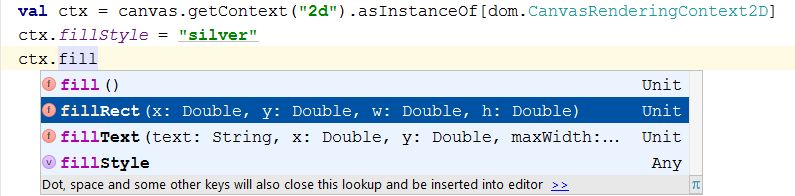
\includegraphics[
    width=1.0\textwidth
%   scale=0.5
    ]{typesafe-autocomplete}
    \caption{Intelligente Auto-Vervollständigung in IntelliJ.
    (Quelle: eigene Anfertigung)
    }
    \label{fig:typesafe-autocomplete}
\end{figure}


	-> Contra (?) bzw. Achtung ->  man muss durch Disziplin selbst darauf achten, dass man js.Dynamic vermeidet und ggf. castet, ist aber selten nötig (-> andere Beispiele???)




\subsubsection{Workbench-Plugin}

Damit das Workbench-Plugin von sbt auch geladen wird, muss es in der \code{plugins.sbt} hinzugefügt werden:

\begin{lstlisting}[style=snippet]
addSbtPlugin("com.lihaoyi" % "workbench" % "0.2.3")
\end{lstlisting}

In der build.sbt müssen folgende Einträge hinzugefügt werden:
\begin{lstlisting}[style=snippet]
workbenchSettings

bootSnippet := "frenzy.CanvasApp().main();"

updateBrowsers <<= updateBrowsers.triggeredBy(fastOptJS in Compile)
\end{lstlisting}

Das \code{bootSnippet} legt fest, welcher JavaScript als Einsprungspunkt für das Neuladen verwendet werden soll. Manchmal genügt ein \code{updateBrowsers} nicht, für solche Fälle existiert das radikalere:

\begin{lstlisting}[style=snippet]
refreshBrowsers <<= refreshBrowsers.triggeredBy(fastOptJS in Compile)
\end{lstlisting}

Nun muss die Workbench noch in der Entwicklungsversion des HTML-Dokuments eingebunden werden durch folgenden Code-Schnipsel:

\begin{lstlisting}[language=HTML5, style=snippet]
<script src="/workbench.js"></script>
\end{lstlisting}

Hierbei ist es wichtig, darauf zu achten, dass diese Zeile nach allen anderen JavaScript-Einbindungen ganz am Ende im \html{<body>} steht.

Beim Start von sbt wird nun automatisch das Workbench-Plugin geladen. Dieses startet einen lokalen Server für das Projektwurzelverzeichnis unter der Adresse \url{localhost/127.0.0.1:12345}. Dadurch ist mit der Eingabe der Adresse \url{http://localhost:12345/target/scala-2.11/classes/index-dev.html} im Browser die Scala.js-Anwendung erreichbar.

Zur flüssigen Entwicklung ist es am komfortabelsten, im kontinuierlichen Modus zu arbeiten. Dazu wird nun \code{\~fastOptJS} aufgerufen, wodurch jedes Speichern von Code-Änderungen einen Build triggert. Ist hierbei die Workbench gestartet, muss das Terminal während der Entwicklung seltener aufgesucht werden, denn selbst Ausgaben des Compilers werden nützlicherweise in der Browser-Konsole ausgegeben (siehe Abb. \ref{fig:workbench-in-action1} - \ref{fig:workbench-in-action4}).

\begin{figure}[!h]
    \centering
    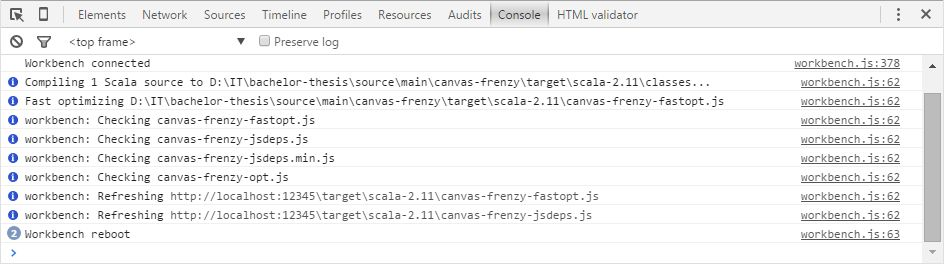
\includegraphics[
    width=1.0\textwidth
%   scale=0.5
    ]{workbench-in-action1}
    \caption{Ausgabe des Scala.js-Compilers in der Browser-Konsole.
    (Quelle: eigene Anfertigung)
    }
    \label{fig:workbench-in-action1}
\end{figure}

\begin{figure}[!h]
    \centering
    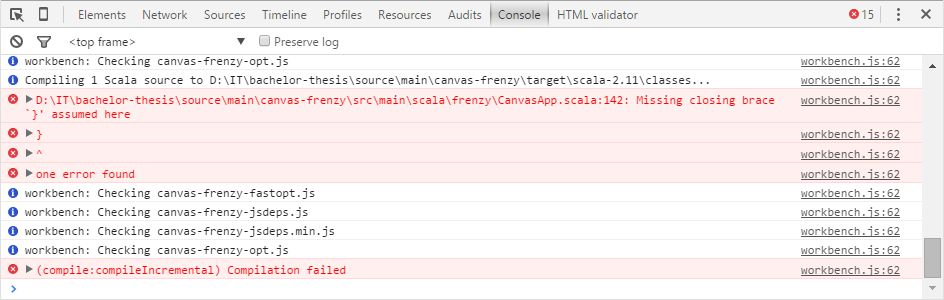
\includegraphics[
    width=1.0\textwidth
%   scale=0.5
    ]{workbench-in-action2}
    \caption{Fehlerausgabe des Scala.js-Compilers in der Browser-Konsole.
    (Quelle: eigene Anfertigung)
    }
    \label{fig:workbench-in-action2}
\end{figure}

Das Workbench-Plugin funktioniert nicht immer ganz zuverlässig, und manchmal muss das Browserfenster per Hand neu geladen werden. Alles in allem ist es aber ein sehr hilfreiches Entwicklungswerkzeug für ein flüssigeres Arbeiten.


















% % % % % % % % % % % % % % % % % % % % % % % % % % % % % % % %
%\section{scalajs-showcase - der Rest:  umfangreichere Templates, Events (3)}
%
%\subsection{Untersuchungsziele}
%\subsection{Untersuchungskriterien}
%\subsection{Kurzbeschreibung des Beispielprogramms}
%\subsection{Untersuchungsergebnisse}
%\subsection{Schwierigkeiten}
%\subsection{Erfolge}
%\subsection{Bewertung: differenziert oder boolsch mit Begründung; Fazit aus Schwierigkeiten und Erfolgen}



% % % % % % % % % % % % % % % % % % % % % % % % % % % % % % % %
\section{Textanalyzer - ein umfangreicheres Beispiel}

%TODO#############################

\subsection{Ziel der Untersuchung}
\subsection{Untersuchungskriterien}
\subsection{Kurzbeschreibung des Beispielprogramms}
\subsection{Ergebnisse der Untersuchung und Bewertung}
\subsection{Schwierigkeiten}
\subsection{Erfolge}
\subsection{Bewertung: differenziert oder boolsch mit Begründung; Fazit aus Schwierigkeiten und Erfolgen}



% % % % % % % % % % % % % % % % % % % % % % % % % % % % % % % %
\section{Ajax: Currency Converter}

%TODO#############################

\subsection{Ziel der Untersuchung}

Die Kommunikation mit Objekten ((?)) außerhalb des Web-Clients, wie zum Beispiel mit Webservices, ist ein wichtiger Bestandteil der allermeisten interaktiven Web-Anwendungen. Dazu wird standardmäßig eine als \textit{Ajax} bezeichnete Technik verwendet. Dabei werden aus der Web-Anwendung heraus über das HTTP-Protokoll Daten von einem Server angefragt, um auf Grundlage der Antwort Teile der HTML-Seite zu aktualisieren. Diese Standardtechnik und die Behandlung von Asynchronität mit Scala.js sollte erprobt werden.

\subsection{Untersuchungskriterien}

\begin{enumerate}
	\item Konfigurationsaufwand
	\item Umsetzbarkeit aller Anforderungen
	\item Leichtigkeit der Implementierung
	\item Code-Qualität (Typsicherheit, Lesbarkeit, Wartbarkeit)
\end{enumerate}

\subsection{Kurzbeschreibung des Beispielprogramms}

Beispielhaft wurde ein Währungsumrechner umgesetzt, der dem Benutzer die Eingabe des Betrags und die Auswahl von Quell- und Zielwährung per Auswahlliste anbietet, und auf Knopfdruck oder Betätigung der Entertaste hin die Umrechnung auf der Basis tagesaktueller Kurse durchführt. Beträge werden bis auf vier Nachkommastellen hin genau dargestellt. Die Eingabe ist fehlertolerant gegenüber ungültigen Beträgen. Als kleiner Komfort kann der Betrag mit der Escape-Taste auf 1.0000 zurückgesetzt werden.

\begin{figure}[!h]
    \centering
    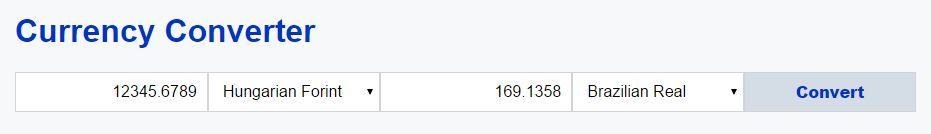
\includegraphics[
    width=1.0\textwidth
%   scale=0.5
    ]{currency-converter/currency-converter}
    \caption{Der Währungsumrechner.
    (Quelle: eigene Anfertigung)
    }
    \label{fig:converter}
\end{figure}

\subsection{Ergebnisse der Untersuchung und Bewertung}

Ist das Setup einer einfachen Scala.js-Anwendung einmal erprobt, bleibt der weitere Konfigurationsaufwand für diese Anwendung gering: die benötigten Bibliotheken müssen lediglich als \code{libraryDependencies} in der Build-Definition hinzugefügt werden.

Das Umrechnungsformular lässt sich mit ScalaTags sehr übersichtlich und deklarativ schreiben. Es werden zwei nahezu identische Währungsauswahllisten benötigt, mit einem Unterschied: Der Auswahlwert soll einmal als Quell-, das andere Mal als Zielwährung behandelt werden. Wir formulieren eine Methode \scala{setupCurrencySelect}, die Auswahllisten erzeugt (Listing \ref{code:setupCurrencySelect}).

\begin{lstlisting}[language=Scala, caption={Methode zur Erzeugung eines \html{<select>}-Elements.}, label={code:setupCurrencySelect}]
def setupCurrencySelect(theId: String,
                        updateConverter: String => Unit,
                        defaultOption: String = "EUR"): html.Select = {
  val sel = select(
    id:=theId,
    for ((code, name) <- Converter.currencies.toSeq) yield option(
      id:=s"$theId-opt-${code.toLowerCase}",
      value:=code, name
    )
  ).render
  sel.onchange = (e: dom.Event) => updateConverter(sel.value)
  sel.value = defaultOption
  sel
}
\end{lstlisting}

Dieser Methode muss eine Funktion \scala{String => Unit} übergeben werden, die den Auswahlwert entgegennimmt, so dass der Umrechner passend aktualisiert werden kann. Die Liste der möglichen \html{<option>}s lässt sich prägnant mithilfe einer \scala{for}-Comprehension ausdrücken. Das Auswahllisten-Elemente, bei dem es sich um ein \scala{scalatags.JsDom.TypedTag[html.Select]} handelt, muss durch Aufruf der Methode \scala{render} in den Fassadentyp \scala{html.Select} der Scala-js-dom-Bibliothek umgewandelt werden. Dadurch haben wir vollen, typsicheren Zugriff auf die Methoden und Attribute ((die in der DOM-API spezifiziert sind)). Ein \scala{onchange}-Handler ließe sich eigentlich auch innerhalb des \scala{select()}-Tags schreiben, allerdings ließe sich so nicht auf das \scala{value}-Attribut zugreifen.

Nach dieser Vorbereitung kann das Umrechnungsformular sehr übersichtlich und deklarativ geschrieben werden (Listing \ref{code:currency-converter-gui}).

\begin{lstlisting}[language=Scala, caption={Deklaration eines Formulars zur Währungsumrechnung mit ScalaTags.}, label={code:currency-converter-gui}]
container.appendChild(
  div(
    h1("Currency Converter"),
    form(
      onsubmit:={ (evt: dom.Event) => evt.preventDefault() },
      inputAmount,
      setupCurrencySelect("sel-src-curr", c => converter = converter.copy(srcCurr = c)),
      outputAmount,
      setupCurrencySelect("sel-dst-curr", c => converter = converter.copy(dstCurr = c)),
      button(
        cls:="input-btn",
        "Convert",
        onclick:={ () => updateDstAmount() }
      )
    )
  ).render
)
\end{lstlisting}

Die Felder für Eingabe (\scala{inputAmount}) und Ergebnis (\scala{outputAmount}) wurden zuvor definiert und mit \scala{.render} umgewandelt, damit sie im Programm referenziert werden können. Auf diese Art ist es nicht nötig, den Umweg über \scala{document.getElementById()} oder mit jQuery-Selektoren zu gehen.

Für die Umrechnung wurde eine Klasse \scala{Converter} definiert. Als Quelle für die Umrechnungskurse sollte die Yahoo! Finance API\footnote{\url{https://code.google.com/p/yahoo-finance-managed/wiki/YQLAPI}} genutzt werden, die auf HTTP-Anfrage hin Ergebnisse im JSON-Format\footnote{JavaScript Object Notation, ein kompaktes Format zum Datenaustausch.} liefert. Anfragen werden in einer Query-Language formuliert. Die Anfrage:

\begin{lstlisting}[aboveskip=0pt, style=snippet]
http://query.yahooapis.com/v1/public/yql?q=select * from yahoo.finance.xchange where pair in ('EURUSD')&format=json&env=store://datatables.org/alltableswithkeys
\end{lstlisting}

liefert als Resultat:

\begin{lstlisting}[language=JavaScript, style=snippet]
{
  "query": {
    "count": 1,
    "created": "2015-10-25T12:58:36Z",
    "lang": "de",
    "results": {
      "rate": {
          "id": "EURUSD",
          "Name": "EUR/USD",
          "Rate": "1.1018",
          "Date": "10/24/2015",
          "Time": "11:55am",
          "Ask": "1.1022",
          "Bid": "1.1013"
      }
    }
  }
}
\end{lstlisting}

Um HTTP-Requests mit Scala.js zu realisieren gibt es verschiedene Möglichkeiten\cite[\#UsingWebServices]{haoyi.HOS}.

Dank Scala-js-dom kann das \code{XMLHttpRequest}-Objekt\footnote{Eine ursprünglich von Microsoft entwickelte API zur Client-Server-Kommunikation, die von den großen Browserherstellern Mozilla, Apple, and Google unterstützt und gegenwärtig vom W3C standardisiert wird.\cite{mdn.XHR}} ganz ähnlich wie mit reinem Java-Script verwendet werden (allerdings typsicher).

\begin{lstlisting}[language=Scala, caption={HTTP-Aufruf mit XMLHttpRequest.}]
val xhr = new dom.XMLHttpRequest()
xhr.open("GET", url)
xhr.onload = (e: dom.Event) => {
  if (xhr.status == 200) {
    handleXhrResponse(xhr)
  }
}
xhr.send()
\end{lstlisting}

Der \scala{onload}-Handler wird als anonyme Funktion übergeben, semantisch ganz analog zu JavaScript:

\begin{lstlisting}[language=JavaScript, style=snippet]
xhr.onload = function(e) { /* ... */ } // JavaScript
\end{lstlisting}

\code{XMLHttpRequest} verlangt relativ viel Handarbeit, bietet aber dafür einen sehr direkten Zugriff auf das HTTP-Protokoll. Für viele Anwendungsfälle ist das jedoch gar nicht nötig. Damit diese prägnanter geschrieben werden können, bietet Scala-js-dom Bequemlichkeitsmethoden für die gebräuchlichsten HTTP-Methoden (GET, POST, PUT und DELETE). Diese Methoden geben eine \scala{Future[dom.XMLHttpRequest]}\footnote{Futures in Scala: \url{http://docs.scala-lang.org/overviews/core/futures.html}} zurück. Damit Futures und Promises in Scala.js verwendet werden können, wird ein Ausführungskontext benötigt.. \cite[\#Extensions]{scala-js-dom.DOC} Zwei zusätzliche Importe sind nötig, der GET-Aufruf schrumpft dafür auf einen Einzeiler:

\begin{lstlisting}[language=Scala, caption={Futures-basierter HTTP-Aufruf mit Scala.js-Bequemlichkeitsmethode.}]
import dom.ext.Ajax
import scalajs.concurrent.JSExecutionContext.Implicits.runNow
Ajax.get(url).onSuccess{ case xhr => handleXhrResponse(xhr) }
\end{lstlisting}

So definieren wir eine \scala{Converter}-Klasse, die immutable ist. Für jedes Währungspaar soll ein neue Instanz erzeugt werden.

\begin{lstlisting}[language=Scala, caption={Der Währungsumrechner.}]
case class Converter(
  srcCurr: String = "EUR",
  dstCurr: String = "EUR"
) {
  def convert(srcAmount: Double): Future[Double] = async{
    srcAmount * await{ rate }
  }

  private def url = "http://query.yahooapis.com/v1/public/yql?q=select * from yahoo.finance.xchange where pair in ('" + srcCurr + dstCurr + "')&format=json&env=store://datatables.org/alltableswithkeys"

  private lazy val rate: Future[Double] = Ajax.get(url).map{ case xhr =>
    val json: js.Dynamic = js.JSON.parse(xhr.responseText)
    json.query.results.rate.Rate.toString.toDouble
  }
}
\end{lstlisting}

Durch den Aufruf von \scala{JSON.parse} wird der Antworttext deserialisiert. Dabei erhalten wir ein dynamisch getyptes Objekt. Hier muss nun besonders sorgfältig vorgegangen werden, da der Compiler uns nicht vor Tippfehlern schützt. Die Rate muss zur sinnvollen Verwendung zuerst in einen String, und dieser dann in einen \scala{Double}-Wert umgewandelt werden.

Nun können wir eine Methode schreiben, die auf Knopfdruck hin eine HTTP-Anfrage beim Webservice stellt und beim Eintreffen der Antwort dafür sorgt, dass der umgerechnete Betrag auf der Webseite angezeigt wird.

\begin{lstlisting}[language=Scala, style=snippet]
def updateDstAmount(): Unit = converter.convert(srcAmount).onSuccess{
  case dstAmount => outputAmount.textContent = format(dstAmount)
}
\end{lstlisting}

Zur Formatierung des Ausgabewerts \scala{dstAmount: Double} muss \scala{\"\%.4f\".format(dstAmount)} oder \scala{f\"\$dstAmount\%.4f\"} verwendet werden, denn die Java-Methode \scala{String.format()} funktioniert nicht. ((DUBLETTE)) Es ist wäre hier auch möglich, durch den Import von \scala{scala.scalajs.js.JSNumberOps.\_}
auf native JavaScript-Methoden zurückzugreifen und \scala{dstAmount.toFixed(4)} zu schreiben.

>>>
- Anforderungen können umgesetzt werden
- Muster müssen gelernt / verstanden werden
- Doku sehr hilfreich, wichtige Orientierung für die beschriebene Implementierung -> vgl. Using Web Services \cite[\#UsingWebServices]{haoyi.HOS}
- dann komfortabel zu benutzen, erhöht Lesbarkeit durch Prägnanz




% % % % % % % % % % % % % % % % % % % % % % % % % % % % % % % %
%\section{js-interop -> playground(?) (3)}
%
%\subsection{Ziel der Untersuchung}
%\subsection{Untersuchungskriterien}
%\subsection{Kurzbeschreibung des Beispielprogramms}
%\subsection{Ergebnisse der Untersuchung und Bewertung}
%\subsection{Schwierigkeiten}
%\subsection{Erfolge}
%\subsection{Bewertung: differenziert oder boolsch mit Begründung; Fazit aus Schwierigkeiten und Erfolgen}

% % % % % % % % % % % % % % % % % % % % % % % % % % % % % % % %
\section{Eine Cross-kompilierende Library: Crosscompiling-statistics-lib}

%TODO#############################

\subsection{Ziel der Untersuchung}
Cross-compiling lib
Performance-Vergleich zu reinem JS - Micro-Benchmark
BILD -> \cite[Folie 52, Min. ???]{doeraene2015.SSP} % -->  Doeraene2015-Scalajs-p52.jpg

\subsection{Untersuchungskriterien}
\subsection{Kurzbeschreibung des Beispielprogramms}
\subsection{Ergebnisse der Untersuchung und Bewertung}


% % % % % % % % % % % % % % % % % % % % % % % % % % % % % % % %
\section{Minimales Client/Server-Setup mit Routing: Clientserver}

%TODO#############################

\subsection{Ziel der Untersuchung}
eine (!) Templating-Sprache für Server und Client: ScalaTags \cite{haoyi.HOS}
eine (!) Library zur Serialisierung: uPickle \cite{haoyi.HOS}
Schnittstelle in einer Sprache

\subsection{Untersuchungskriterien}
\subsection{Kurzbeschreibung des Beispielprogramms}
entsprechend Code-Vorschlägen von Li Haoy\cite{haoyi.HOS}
\subsection{Ergebnisse der Untersuchung und Bewertung}


ggf. diskutieren: Verwendung vieler objects

- muss nicht zwei Libraries für Client und Server finden
- leichter nur eine (!) Library (jeweils für Templating und Serialisierung) zu lernen, die in Client und Server verwendet werden kann
\cite[\#SharingCode]{haoyi.HOS}
- relativ einfache statisch typisierte RPCs mit autowire


% % % % % % % % % % % % % % % % % % % % % % % % % % % % % % % %
%\chapter{Auswertung (speziell der "`weichen"' Kriterien)}


% % % % % % % % % % % % % % % % % % % % % % % % % % % % % % % %
\chapter{Fazit}

\section{Zusammenfassung der Ergebnisse}

TODO - NACH FERTIGSTELLUNG DER ÜBRIGEN KAPITEL NEU SCHREIBEN!

   Korrektheit
	-> doeraene TDI S.7, links
   Performance
	--> doeraene TDI S. 7, oben rechts
	(-> eigenes Micro-Benchmark -> Bsp.)
>> Nützlichkeit
	- getypter DOM
	- getypte Fassaden für jQuery und Libs
	- bei Bedarf: js.Dynamic

Die vorliegende Arbeit ...
- Überblick über Entwicklung von Weboberflächen mit Scala.js
- Eignung aus Anwendersicht ...
- Eignung aus Entwicklersicht ...
- Vorteile ...
	- vollständiger Scala-Support
	- umfassende JS-Interop
	- sbt-Integration
	- Typsicherheit
		- weniger Fehler
		- IDE-Support!
	- Sourcemaps zum besseren Debugging
- Nachteile ...
	- noch etwas große Kompilate

Pro Scala.js:
    - direkt mit dem DOM arbeiten, aber getypt
    - zwischen Client/Server geteilt: Konstanten, Algorithmen, Datenstrukturen, Libraries
    - Typsicherheit
    - Interface zwischen Client/Server
    - Scala-Programmierer können ohne die Sprache zu wechseln fürs Web programmieren
    - inkrementelle Kompilation, DCE (Dead code elemination)
Contra Scala.js:
    - small Community
    - kleines Entwicklerteam, keine Unterstützung durch ein größere Firma
    - langsamer Scala-Compiler
    - große Bibliothek --> relativ große Kompilate





>> was spricht für Scala.js?
    nach nicht-repräsentativer Umfrage (
      vgl.  -->  \url{http://www.scala-lang.org/news/2015/02/05/scala-js-no-longer-experimental.html}
      Diskussion hier  -->  \url{https://groups.google.com/forum/#!topic/scala-js/_1Sfb5Nj08w}
    ):
    - geteilter Code zwischen Client und Server, eine Sprache für die gesamte Anwendung, z.B. für Validierungs-Logik, aber auch Wiederverwendbarkeit von Code (wenn keine Plattformspezifika direkt verwendet werden)
    \cite{doeraene2013.CSJ}
    - starke Typisierung, auch für JavaScript-Libraries
    - Tooling: IDE-Support, sbt-Integration, Dependency-Management, Unit-Tests, Stacktraces und Sourcemaps, kross-compilierende Projekte
    - Portababilität: Scala auf JavaScript-basierten Plattformen

  kompletter Scala-Support
  
  schnelle Ints:
  - Int-Operationen werden durch bitweise Veroderung umgesetzt (z.B. Scala.js: a + b -> JS: (a + b) | 0)
  - JS VMs verwenden intern int32 als Optimierung für bitweise Operationen
  -> schneller\cite{doeraene2015.SSP}


  schneller Dev-cycle, optim. Prod.code
  
  Scala im Browser!!!
  
  
was fehlt?
  (- checked Exceptions???)
  (- Regex???)
  - Unterstützung von Laufzeit-Reflection

Schwächen
  - relativ große Dateien
  (- Debugging schwieriger???)
  - Support für einige Libraries
  - Performance
  
Unbequemlichkeiten
  - Auslieferung von Produktionscode noch etwas mühsam: kompiliert nach
\begin{lstlisting}
target/
  +- scala-2.11/
  +- [...]-opt.js
  +- [...]-jsdeps.min.js
  +- classes/
      +- index.html
      +- [...].css
\end{lstlisting}
  - muss per Hand extrahiert werden
  - wenn andere Ordnerstruktur gewünscht ist, z.B.:
\begin{lstlisting}
webapp/
 +- js/
 |   +- [...]-opt.js
 |   +- [...]-jsdeps.min.js
 +- css/
 |   +- [...].css
 +- index.html
\end{lstlisting}
  ... dann müssen die Pfade in der index.html entsprechend geändert werden
  -> Lösung wären hier entsprechende Export-Skripte; bzw. denkbar, dass in Zukunft ein entsprechendes Tool oder sbt-Plugin (?) angeboten wird



großes Potential
	besonders weil: eine Sprache für Client und Server
		Wiederverwendbarkeit von Code
		nur in einer Sprache denken, nicht eine weitere lernen
	typbedingte Laufzeitfehler auch für Client-Seite (JavaScript) ausgeschlossen sind
	mit Templating-Library auch HTML-Tags typsicher macht
	
Doku noch im Wandel, stellenweise ("`tiefer drin"') noch etwas sparsam erklärt, zeitweise und sporadisch nicht mit den neuesten Änderungen synchron, aber im Großen und Ganzen ziemlich gut

vor allem für Entwickler und Projekte die schon mit Scala arbeiten sehr interessant

Erfolg hängt sicher auch am Erfolg der Sprache Scala
dafür, dass noch sehr jung, schon sehr gut entwickelt und anscheinend stabil




Hürden

- speziellere Konfiguration, besonders
  - für Cross-Projekte
  - vermutlich, wenn Vorgaben für die zu verwendenden Techniken bestehen

Chancen

- eine eindeutige, typsichere Schnittstelle zur Client-Server-Kommunikation





\section{Ausblick}

TODO - NACH FERTIGSTELLUNG DER ÜBRIGEN KAPITEL NEU SCHREIBEN!

Blick über den Tellerrand:
- anderer vielversprechender Ansatz: Elm
	-->  \url{http://elm-lang.org/}
	- FRP (Functional Reactive Programming) Sprache um deklarativ UIs für den Browser zu schreiben, statisch typisiert
	- kompiliert nach HTML, CSS und JavaScript
	- hat REPL, package manager, debugger
	- libraries
	- Alternative zu Scala.js? - kein Scala, nur Client...



Weiterentwicklung

	ganz neu (aber nicht untersucht): \url{http://www.scala-js.org/doc/sjs-defined-js-classes.html}
	SJS-Klassen von JS-Klassen erben lassen  -->  \url{https://github.com/scala-js/scala-js/issues/1795}
	
	
	angekündigt: volle Unterstützung von runtime reflections\cite[S. 2]{doeraene2013.TDI}
	angekündigt: eventuell Compiler im Browser\cite[Folie 39, Min. 39]{doeraene2014.WHB}
	angekündigt: vollwertige Akka-Aktoren\cite[Folie 39, Min. 39]{doeraene2014.WHB}
	



professionelle Anwendungen mit Scala.js

		https://jaxenter.com/happy-tenth-birthday-scala-whats-next-107440.html
	https://jaxenter.de/scala-javascript-compiler-scalajs-0-6-0-produktionseinsatz-13633
	- die Frage ist, ob Frontend/Client-side-Entwickler bereit sind, auf Scala.js umzusteigen (ohne vorherige Scala-Kenntnisse, und die sind i.d.R. nicht anzunehmen), aber es könnte ein großer Gewinn sein: Vorteile mit Scala zu arbeiten\cite{doeraene2013.CSJ}




Ausblick
  - (hoffentlich) schnell (?) wachsender Library-Support, 
     	- gerade wegen der Erweiterbarkeit von Scala auch bei kleiner (aber reger und enthusiastischer) Scala.js-Community  recht wahrscheinlich
  - Performance-Verbesserungen
  - professioneller Einsatz?
    -->  \url{https://www.reddit.com/r/scala/comments/2spdlq/is_anyone_using_scalajs_in_nontrivial/}





% % % % % % % % % % % % % % % % % % % % % % % % % % % % % % % %

\appendix
\chapter{Quellcodeauszüge usw.}

\section{Beispielabbildung}

blabla (siehe Abb. \ref{fig:a_picture_of_tux}) blabla

\begin{figure}[!h]
    \centering
    
\includegraphics[
    width=0.25\linewidth
%   scale=0.5
    ]{tux}
    \caption{Eine Beispielabbildung.
    (Quelle: \cite{aab.FBB})
    }
    \label{fig:a_picture_of_tux}
\end{figure}

blabla


\section{Beispielcode}

blabla \verb|println(this)| blabla

blablba \verb|var sqr = function(x) { return x * x; }| blabla

\verb|var sqr = function(x) { return x * x; }|

\begin{verbatim}
var sqr = function(x) { return x * x; }
for (var i = 0; i < 10; i++) {
  console.log(i, sqr(i));
}
\end{verbatim}

% possible to emph and textbf, but curly braces have to be escaped:
\begin{alltt}
var \emph{sqr} = function(x) \{ \textbf{return} x * x; \}
for (var i = 0; i < 10; i++) \{
  console.log(i, \emph{sqr}(i));
\}
\end{alltt}


Ein kleines JavaScript-Codeschnipsel könnte man \lstinline[language=JavaScript, style=inline]!function(x) { return 2 + x; }! inline schreiben. Und ein kleines Scala-Codeschnipsel könnte man \lstinline[language=Scala, style=inline]|def foo(): Unit = println("bar")| inline schreiben.


\begin{lstlisting}
var sqr = function(x) { return x * x; }
for (var i = 0; i < 10; i++) {
  console.log(i, sqr(i));
}
\end{lstlisting}

Some Python code:
\lstinputlisting[language=Python, xleftmargin=10pt, caption={This is just a Python example}]{listings/example.py}


% % % % % % % % % % % % % % % % % % % % % % % % % % % % % % % %


Some Scala code:
\lstinputlisting[language=Scala, caption={And this is a very stupid Scala example}]{listings/example.scala}

And again some Scala code:
\lstinputlisting[language=Scala, linerange={3-6,16-31}, style=uncolored, style=numbered, caption={An excerpt from the very same example}]{listings/example.scala}


% % % % % % % % % % % % % % % % % % % % % % % % % % % % % % % %


Some JavaScript code:
\lstinputlisting[language=JavaScript, caption={A JavaScript example}, firstline=3, lastline=39, style=unframed, style=numbered, frame=single, rulecolor=\color{blue}]{listings/example.js}


% % % % % % % % % % % % % % % % % % % % % % % % % % % % % % % %


Some HTML code with line numbers:
\lstinputlisting[language=HTML5, style=numbered, caption={And finally a HTML example}]{listings/example.html}


% % % % % % % % % % % % % % % % % % % % % % % % % % % % % % % %
% % % % % % % % % % % % % % % % % % % % % % % % % % % % % % % %




% ABBILDUNGSVERZEICHNIS ERSTELLEN
\listoffigures

% TABELLENVERZEICHNIS ERSTELLEN
\listoftables

% QUEELLCODEVERZEIHCHNIS ERSTELLEN
\lstlistoflistings

% LITERATURVERZEICHNIS ERSTELLEN
%\begin{thebibliography}{xxxxxxxxxxxxxxxxxxx}
%   \bibitem[BECK, ????]{BECK} Beck, Kent: Extreme Programming : Das Manifest, Addison-Wesley, ORT, JAHR. % TODO
%   \bibitem[ARIS, ????]{ARIS} Arisholm, Erik; Gallis, Hans; Dyb\aa , Tore; Sj\o berg, Dag I.K.: TITEL. In: IEEE Transcactions on Software
%    Engineering, Vol. 33, No. 2, Februar 2007.
%
%
%
%   \bibitem[GoF, 1994]{GoF1} Erich Gamma, Richard Helm, Ralph Johnson, John Vlissides: Design Patterns: Elements of reusable object oriented software Addison Wesley Publishing Company 1994, ISBN 0-201-63361-2
%   \bibitem[BMBF, 2003]{bmbf}"'IT-Ausstattung der allgemein bildenden und berufsbildenden Schulen in Deutschland"', http://www.schulen-ans-netz.de/neuemedien/fakten/dokus/it-ausstattung-2003.pdf, 10.03.2005
%\end{thebibliography}


% TODO: nocite entfernen, damit nur zitierte Literatur ins Verzeichnis kommt
\nocite{*}


% Bibliographie mit bibtex
%\bibliographystyle{alphadin}
%\bibliography{biblio_scalajs}


% Bibliographie mit biblatex/biber
\printbibliography



%%%%%%%%%%%%%%%%%%%%%%%%%%%%%%%%%%%%%%%%%%%%
% END DOCUMENT // HIER HÖRT DER INHALT AUF
%%%%%%%%%%%%%%%%%%%%%%%%%%%%%%%%%%%%%%%%%%%%
\end{document}








